\documentclass{beamer}
\usepackage[utf8]{inputenc}
\usepackage{graphicx, epsfig}
\usepackage{amsmath,mathrsfs,amsfonts,amssymb}
%\usepackage{subfig}
\usepackage{floatflt}
\usepackage{epic,ecltree}
\usepackage{mathtext}
\usepackage{fancybox}
\usepackage{fancyhdr}
\usepackage{multirow}
\usepackage{enumerate}
\usepackage{epstopdf}
\usepackage{multicol}
\usepackage{algorithm}
\usepackage[noend]{algorithmic}
\def\algorithmicrequire{\textbf{Input:}}
\def\algorithmicensure{\textbf{Output:}}
\usetheme{default}%{Singapore}%{Warsaw}%{Warsaw}%{Darmstadt}
\usecolortheme{default}
\setbeamertemplate{footline}[page number]{}
\setbeamerfont{title}{size=\Huge}

\newcommand{\ba}{\mathbf{a}} 
\newcommand{\be}{\mathbf{e}} 
\newcommand{\bt}{\mathbf{t}} 
\newcommand{\bu}{\mathbf{u}} 
\newcommand{\bv}{\mathbf{v}} 
\newcommand{\bw}{\mathbf{w}} 
\newcommand{\bx}{\mathbf{x}} 
\newcommand{\bz}{\mathbf{z}} 
\newcommand{\by}{\mathbf{y}} 

\newcommand{\bI}{\mathbf{I}} 
\newcommand{\bT}{\mathbf{T}} 
\newcommand{\bX}{\mathbf{X}} 
\newcommand{\bZ}{\mathbf{Z}} 

\newcommand{\bbR}{\mathbb{R}} 

\newcommand{\bepsilon}{\boldsymbol{\epsilon}}
\newcommand{\bmu}{\boldsymbol{\mu}}
\newcommand{\blambda}{\boldsymbol{\lambda}}
\newcommand{\bsigma}{\boldsymbol{\sigma}}

\newcommand{\btheta}{\boldsymbol{\theta}} 
\newcommand{\bphi}{\boldsymbol{\phi}} 

\DeclareMathOperator*{\argmin}{arg\,min}
\DeclareMathOperator*{\argmax}{arg\,max}

%\definecolor{beamer@blendedblue}{RGB}{15,120,80}
%----------------------------------------------------------------------------------------------------------
\title[\hbox to 56mm{Deep Generative Models  \hfill\insertframenumber\,/\,\inserttotalframenumber}]
{Deep Generative Models \\ Lecture 12}
\author[Roman Isachenko]{\\Roman Isachenko}
\institute[MIPT]{Moscow Institute of Physics and Technology \\
}
\date{2020}
%--------------------------------------------------------------------------------
\begin{document}
%--------------------------------------------------------------------------------
\begin{frame}
%\thispagestyle{empty}
\titlepage
\end{frame}
\begin{frame}{Neural ODE}
\begin{minipage}[t]{0.6\columnwidth}
\vspace{0.2cm}
\begin{itemize}
	\item Neural network for classification task has hundreds of layers.
	\item Skip connections eliminates exploding/vanishing gradients.
\end{itemize}
\[
	\bz_{t + 1} = \bz_t + f(\bz_t, \btheta)
\]
\end{minipage}%
\begin{minipage}[t]{0.4\columnwidth}
\begin{figure}
    \centering
    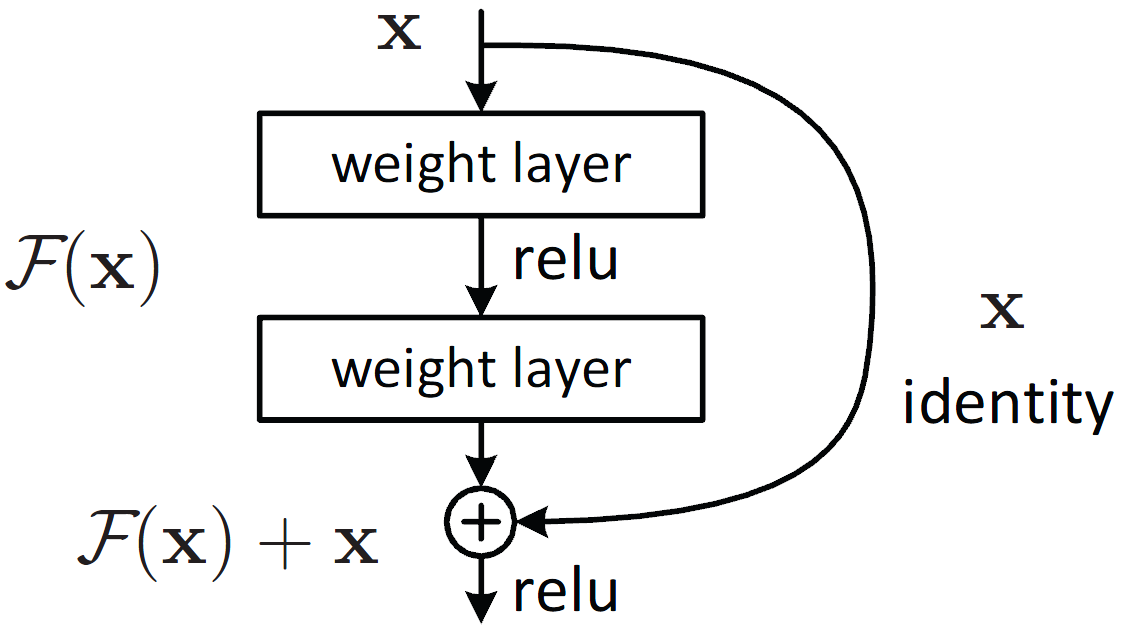
\includegraphics[width=0.95\linewidth]{figs/resnet_1.png}
\end{figure}
\end{minipage}
\begin{figure}
    \centering
    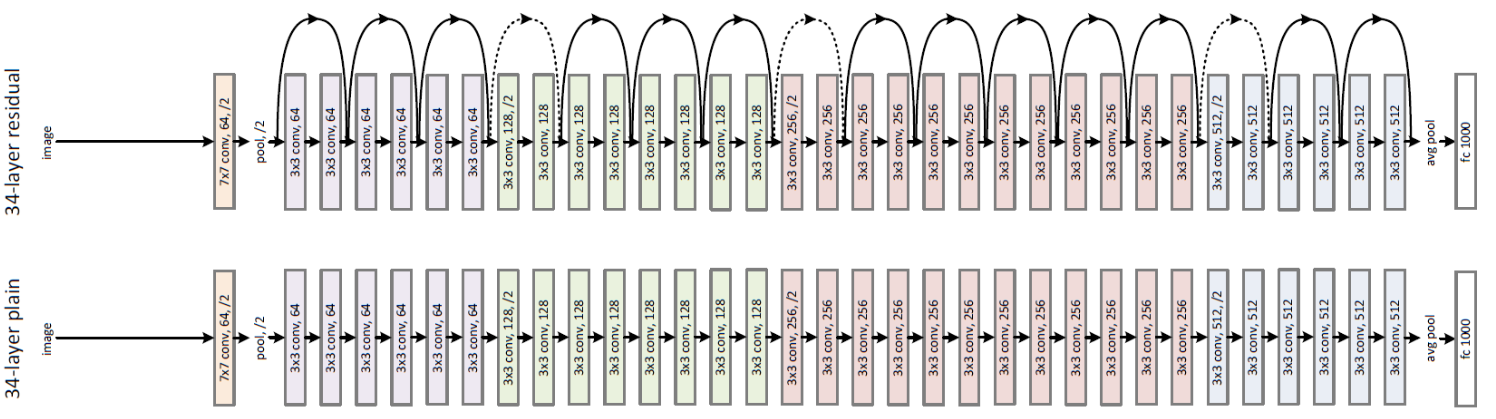
\includegraphics[width=\linewidth]{figs/resnet_2.png}
\end{figure}
\vfill
\hrule\medskip
{\scriptsize \href{https://arxiv.org/abs/1806.07366}{https://arxiv.org/abs/1806.07366}}   
\end{frame}
%=======
\begin{frame}{Neural ODE}
	Consider Ordinary Differential Equation    
	\begin{align*}
	    \frac{d \bz(t)}{dt} &= f(\bz(t), \btheta); \quad \text{with initial condition }\bz(t_0) = \bz_0. \\
	    \bz(t_1) &= \int^{t_1}_{t_0} f(\bz(t), \btheta) d t  + \bz_0 = \text{ODESolve}(\bz(t_0), f, t_0,t_1, \btheta).
	\end{align*}
	\vspace{-0.4cm}
	\begin{block}{Euler update step}
		\vspace{-0.4cm}
		\[
		    \frac{\bz(t + \Delta t) - \bz(t)}{\Delta t} = f(\bz(t), \btheta) \quad \Rightarrow \quad \bz(t + \Delta t) = \bz(t) + \Delta t f(\bz(t), \btheta).
		\]
		\vspace{-0.5cm}
	\end{block}
	\begin{block}{Residual block}
		\vspace{-0.5cm}
		\[
		    \bz_{t+1} = \bz_t + f(\bz_t, \btheta).
		\]
		\vspace{-0.4cm}
	\end{block}
	\begin{itemize}
	 \item Residual learning is equavalent to Euler update step for solving ODE with $\Delta t = 1$!
	 \item Euler update step is unstable and trivial. There are much more sophisticated methods.
	\end{itemize}
	 \vfill
	\hrule\medskip
	{\scriptsize \href{https://arxiv.org/abs/1806.07366}{https://arxiv.org/abs/1806.07366}}   
\end{frame}
%=======
\begin{frame}{Neural ODE}
	\begin{block}{Residual block}
	\vspace{-0.3cm}
	\[
	    \bz_{t+1} = \bz_t + f(\bz_t, \btheta).
	\]
	\vspace{-0.4cm}
	\end{block}
	\begin{itemize}
		\item What happens as we add more layers and take smaller steps? \\
		\item In the limit, we parameterize the continuous dynamics of hidden units using an ODE specified by a neural network: 
	\[
	    \frac{d \bz(t)}{dt} = f(\bz(t), t, \btheta); \quad \bz(t_0) = \bx; \quad \bz(t_1) = \by.
	\]
	\end{itemize}
	\begin{minipage}[t]{0.4\columnwidth}
		\begin{figure}
			\centering
			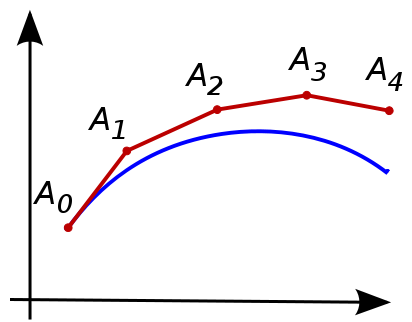
\includegraphics[width=0.9\linewidth]{figs/euler}
		\end{figure}
	\end{minipage}%
	\begin{minipage}[t]{0.6\columnwidth}
		\begin{figure}
			\centering
			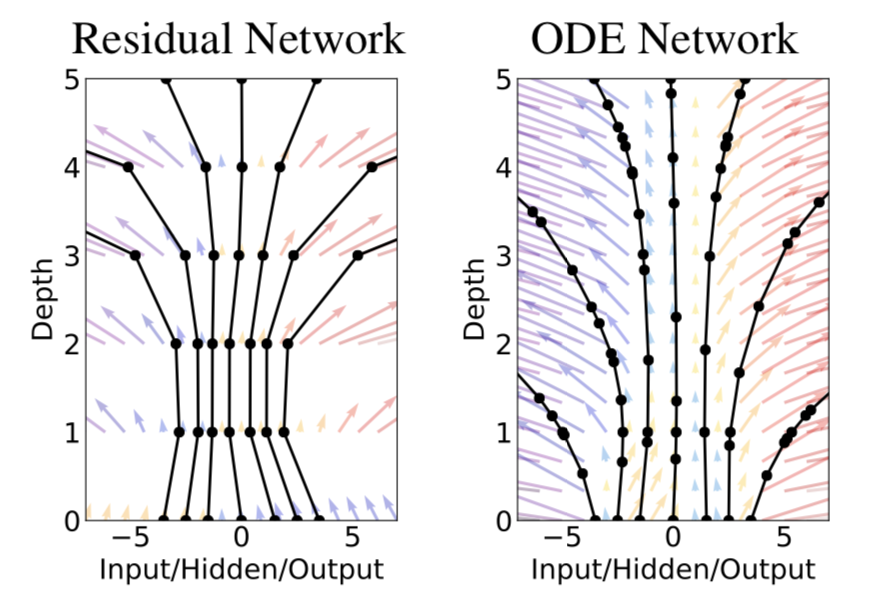
\includegraphics[width=0.8\linewidth]{figs/resnet_vs_neural_ode.png}
		\end{figure}
	\end{minipage}
	\hrule\medskip
	{\scriptsize \href{https://arxiv.org/abs/1806.07366}{https://arxiv.org/abs/1806.07366}}   
\end{frame}
%=======

\begin{frame}{Neural ODE}
	\begin{block}{Forward pass (loss function)}
		\vspace{-0.5cm}
		\begin{align*}
			L(\by) = L(\bz(t_1)) &= L\left( \bz(t_0) + \int_{t_0}^{t_1} f(\bz(t), \btheta) dt \right) \\ &= L\left(\text{ODESolve}(\bz(t_0), f, t_0,t_1, \btheta) \right)
		\end{align*}
	\vspace{-0.5cm}
	\end{block}
	\textbf{Note:} ODESolve could be any method (not neccessary Euler).
	\begin{block}{Backward pass (gradients computation)}
		For fitting parameters we need gradients:
		\[
		\ba_{\bz}(t) = \frac{\partial L(\by)}{\partial \bz(t)}; \quad \ba_{\btheta}(t) = \frac{\partial L(\by)}{\partial \btheta(t)}.
		\]
		In theory of optimal control this functions called \textbf{adjoint} functions. 
		They shows how the gradient of the loss depends on the hidden state~$\bz(t)$ and parameters $\btheta$.
	\end{block}
	\vspace{0.1cm}
		
	\hrule\medskip
	{\scriptsize \href{https://arxiv.org/abs/1806.07366}{https://arxiv.org/abs/1806.07366}}   
\end{frame}
%=======
\begin{frame}{Neural ODE}
	\begin{block}{Loss function (forward pass)}
	\vspace{-0.2cm}
	\[
	    L(\by) = L(\bz(t_1)) = L\left(\text{ODESolve}(\bz(t_0), f, t_0,t_1, \btheta) \right)
	\]
	\vspace{-0.3cm}
	\end{block}
	\begin{block}{Adjoint functions}
	\vspace{-0.2cm}
	\[
	    \ba_{\bz}(t) = \frac{\partial L(\bz(t))}{\partial \bz(t)}; \quad \ba_{\btheta}(t) = \frac{\partial L(\bz(t))}{\partial \btheta}
	\]
	\vspace{-0.2cm}
	\end{block}
	\begin{block}{Theorem (Pontryagin)}
	\vspace{-0.3cm}
	\[
	    \frac{d \ba_{\bz}(t)}{dt} = - \ba_{\bz}(t)^T \cdot \frac{\partial f(\bz(t), \btheta)}{\partial \bz(t)}; \quad  \frac{d \ba_{\btheta}(t)}{dt} = - \ba_{\bz}(t)^T \cdot \frac{\partial f(\bz(t), \btheta)}{\partial \btheta}
	\]
	Do we know any initilal condition?
	\end{block}
	 \vfill
	\hrule\medskip
	{\scriptsize \href{https://arxiv.org/abs/1806.07366}{https://arxiv.org/abs/1806.07366}}   
\end{frame}
%=======
\begin{frame}{Neural ODE}
	\begin{block}{Theorem (Pontryagin)}
		\vspace{-0.3cm}
		\[
		\frac{d \ba_{\bz}(t)}{dt} = - \ba_{\bz}(t)^T \cdot \frac{\partial f(\bz(t), \btheta)}{\partial \bz(t)}; \quad  \frac{d \ba_{\btheta}(t)}{dt} = - \ba_{\bz}(t)^T \cdot \frac{\partial f(\bz(t), \btheta)}{\partial \btheta}
		\]
	\end{block}
	\begin{block}{Solution for adjoint function}
		\begin{align*}
		 \frac{\partial L}{\partial \bz(t_0)} &= \ba_{\bz}(t_0) =  - \int_{t_1}^{t_0} \ba_{\bz}(t)^T \frac{\partial f(\bz(t), t, \btheta)}{\partial \bz(t)} dt + \frac{\partial L}{\partial \bz(t_1)} \\
		 \frac{\partial L}{\partial \btheta(t_0)} &= \ba_{\btheta}(t_0) =  - \int_{t_1}^{t_0} \ba_{\bz}(t)^T \frac{\partial f(\bz(t), \btheta))}{\partial \btheta(t)} dt \\
		 \bz(t_0) &= \int^{t_0}_{t_1} f(\bz(t), \btheta) d t  + \bz_1.
		\end{align*}
	\end{block}
	\vfill
	\hrule\medskip
	{\scriptsize \href{https://arxiv.org/abs/1806.07366}{https://arxiv.org/abs/1806.07366}} 
\end{frame}
%=======
\begin{frame}{Neural ODE}
	\begin{block}{Forward pass}
		\[
		\bz(t_1) = \int^{t_1}_{t_0} f(\bz(t), \btheta) d t  + \bz_0 \quad \Rightarrow \quad \text{ODE Solver}
		\]
	\end{block}
	\begin{block}{Backward pass}
		\small
		\vspace{-0.3cm}
		\begin{equation*}
			{\left.\begin{aligned}
				\frac{\partial L}{\partial \bz(t_0)} &= \ba_{\bz}(t_0) =  - \int_{t_1}^{t_0} \ba_{\bz}(t)^T \frac{\partial f(\bz(t), t, \btheta)}{\partial \bz(t)} dt + \frac{\partial L}{\partial \bz(t_1)} \\
				\frac{\partial L}{\partial \btheta(t_0)} &= \ba_{\btheta}(t_0) =  - \int_{t_1}^{t_0} \ba_{\bz}(t)^T \frac{\partial f(\bz(t), \btheta))}{\partial \btheta(t)} dt \\
				\bz(t_0) &= \int^{t_0}_{t_1} f(\bz(t), \btheta) d t  + \bz_1.
			\end{aligned}\right\rbrace} \Rightarrow
			\text{ODE Solver}
		\end{equation*}
	\end{block}
	\vfill
	\hrule\medskip
	{\scriptsize \href{https://arxiv.org/abs/1806.07366}{https://arxiv.org/abs/1806.07366}} 
\end{frame}
%=======
\begin{frame}{Neural ODE}
	
	\begin{figure}
		\centering
		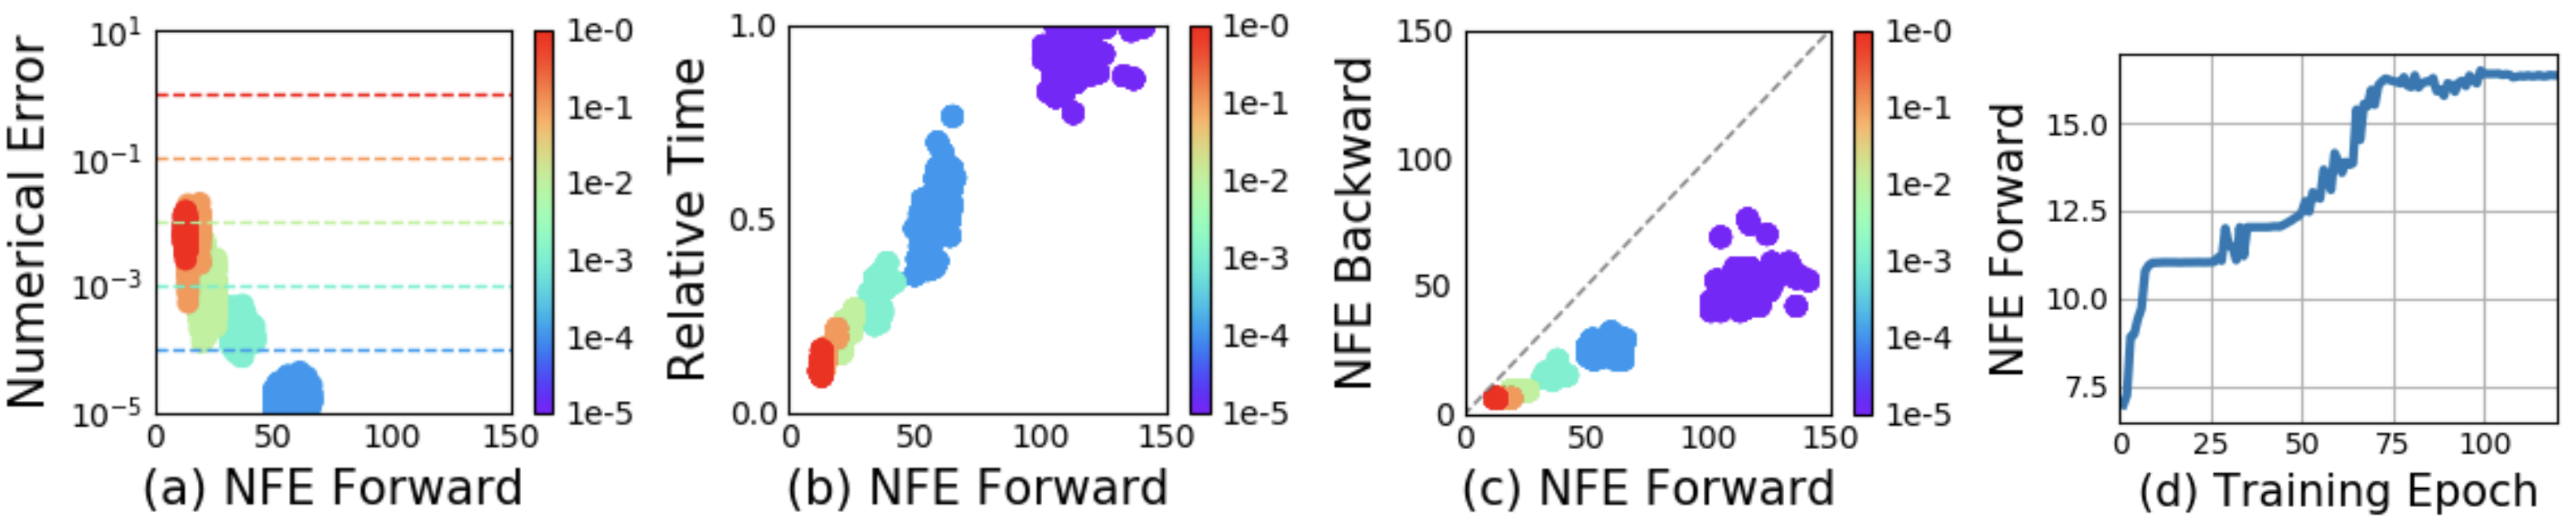
\includegraphics[width=\linewidth]{figs/neural_ode}
	\end{figure}
	
	\begin{block}{Benefits}
		\begin{itemize}
			\item memory efficient (there is no need to store activations);
			\item adaptive computation (depth is not defined explicitly);
			\item parameter efficient (there is only parameters of function $f(\bz(t), \btheta)$);
			\item scalable and invertible normalizing flows (we will discuss it today).
		\end{itemize}
	\end{block}
	\vfill
	\hrule\medskip
	{\scriptsize \href{https://arxiv.org/abs/1806.07366}{https://arxiv.org/abs/1806.07366}}   
\end{frame}
%=======
\begin{frame}{Continuous Normaling Flows}
	\begin{block}{Discrete Normalizing Fflows}
		\vspace{-0.4cm}
		  \[
		  \bz_{t+1} = f(\bz_t, \btheta); \quad \log p(\bz_{t+1}) = \log p(\bz_{t}) - \log \left| \det \frac{\partial f(\bz_t, \btheta)}{\partial \bz_{t}} \right| .
		  \]
		\vspace{-0.4cm}
	\end{block}
	\begin{block}{Planar flows}
		\vspace{-0.3cm}
		\[
		\bz_{t + 1} = g(\bz_t, \btheta) = \bz_t + \mathbf{u} h(\bw^T\bz_t + b) = \bz_t + f(\bz_t, \btheta).
		\]
		Exactly residual learning.
	\end{block}
	Let consider continuous-in-time dynamic transformation of $\bz_t$
	\[
		\frac{d\bz(t)}{dt} = f(\bz(t), \btheta).
	\]
	\vspace{-0.3cm}
	\begin{block}{Continuous dynamic for planar flows}
		\vspace{-0.3cm}
		\[
			\frac{d\bz(t)}{dt}  = \mathbf{u} h(\bw^T\bz_t + b); \quad \frac{\partial \log p (\bz(t))}{ \partial t} = - \mathbf{u}^T \frac{\partial h}{\partial \bz(t)}.
		\]
	\end{block}
	\vfill
	\hrule\medskip
	{\scriptsize \href{https://arxiv.org/abs/1806.07366}{https://arxiv.org/abs/1806.07366}} 
\end{frame}
%=======
\begin{frame}{Continuous Normaling Flows}
	\begin{block}{Theorem}
		Consider the continuous dynamic $\frac{d\bz(t)}{dt} = f(\bz(t), \btheta)$. if function $f$ is uniformly Lipschitz continuous in $\bz$ and continuous in $t$, then the change in log probability follows a differential equation
		\[
		\frac{\partial \log p(\bz(t))}{\partial t} = - \text{trace} \left( \frac{\partial f}{\partial \bz(t)} \right).
		\]
		\vspace{-0.1cm}
		Continuity of function $f$ guarantees that the solution of ODE exists and unique (Piccard theorem).
	\end{block}
	\begin{itemize}
		\item Unlike standard finite flows, the differential equation $f$ does not need to be bijective, since if
		uniqueness is satisfied, then the entire transformation is automatically bijective.
		\item trace($\cdot$) is a linear op instead of det($\cdot$)
		\vspace{-0.1cm}
		\[
		\frac{d\bz(t)}{dt} = \sum_{j=1}^M f_j(\bz(t), \btheta); \quad \frac{\partial \log p(\bz(t))}{\partial t} = - \sum_{j=1}^M\text{trace} \left( \frac{\partial f_j}{\partial \bz(t)} \right).
		\]
	\end{itemize}
	\vfill
	\hrule\medskip
	{\scriptsize \href{https://arxiv.org/abs/1806.07366}{https://arxiv.org/abs/1806.07366}} 
\end{frame}
%=======
\begin{frame}{Continuous NF}
	\begin{block}{Solution for continuous NF}
		\vspace{-0.3cm}
	\begin{align*}
		\bz(t_0) &= \int_{t_1}^{t_0} f(\bz(t), \btheta) dt + \bz(t_1); \\
	    \log p(\bz(t_1)) &= \log p(\bz(t_0)) - \int_{t_0}^{t_1} \text{trace} \left( \frac{\partial f}{\partial \bz(t)} \right) dt.
	\end{align*}
	\end{block}
	\vspace{-0.3cm}
	\begin{figure}
	    \centering
	    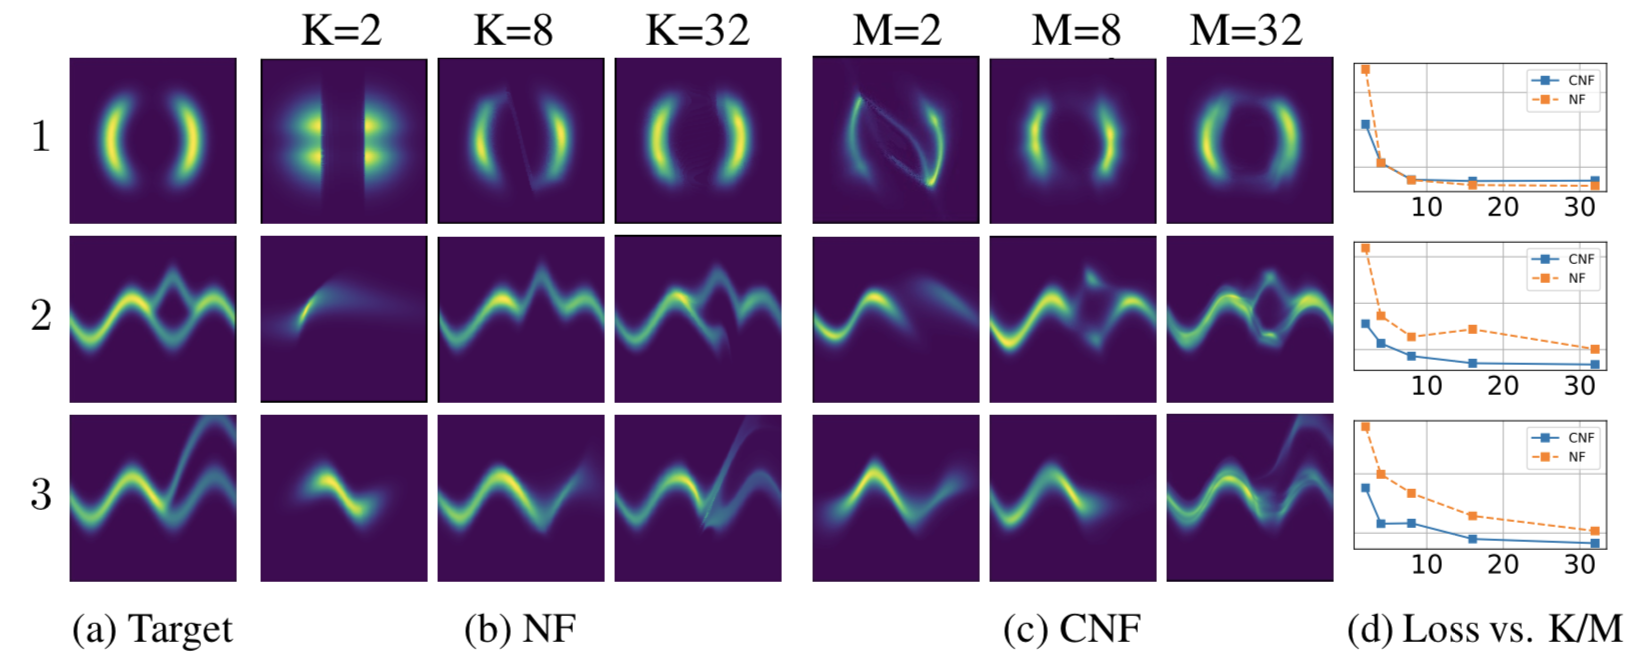
\includegraphics[width=1\linewidth]{figs/cnf}
	\end{figure}
	\vfill
	\hrule\medskip
	{\scriptsize \href{https://arxiv.org/abs/1806.07366}{https://arxiv.org/abs/1806.07366}} 
\end{frame}
%=======
\begin{frame}{Continuous NF}
	
	\begin{minipage}[t]{0.45\columnwidth}
		\begin{itemize}
			\item Standard normalizing flows need invertible $f$.
			\item In general, it costs $O(d^3)$ to get det of Jacobian.
			\item Continuous flows need smooth $f$.
			\item In general, it costs $O(d^2)$ to get trace of Jacobian.
		\end{itemize}
	\end{minipage}%
	\begin{minipage}[t]{0.55\columnwidth}
		\begin{figure}
			\centering
			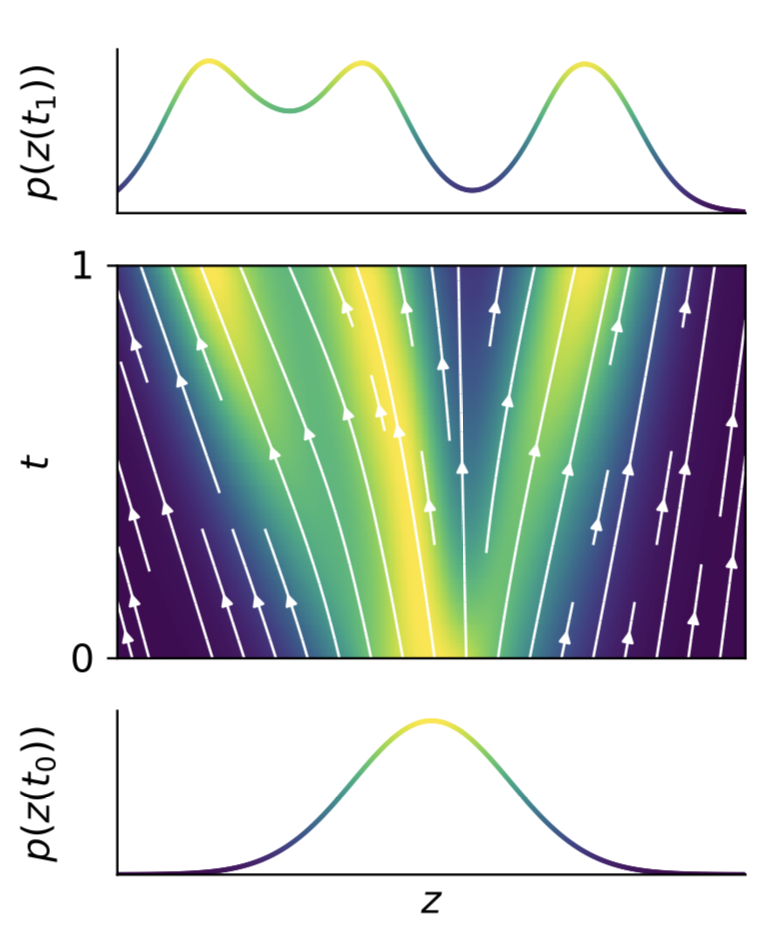
\includegraphics[width=\linewidth]{figs/cnf_flow.png}
		\end{figure}
	\end{minipage}
\vfill
\hrule\medskip
{\scriptsize \href{https://arxiv.org/abs/1806.07366}{https://arxiv.org/abs/1806.07366}} 
\end{frame}
%=======
\begin{frame}{FFJORD}
	It is possible to reduce cost from $O(d^2)$ to $O(d)$.
	\begin{block}{Hutchinson's trace estimator}
	\[
	    \text{trace}(A) = \mathbb{E}_{p(\bepsilon)} \left[ \bepsilon^T A \bepsilon \right]; \quad \mathbb{E} [\bepsilon] = 0; \quad \text{Cov} (\bepsilon) = I.
	\]
	\end{block}
	\begin{block}{Unbiased estimation}
		\vspace{-0.3cm}
	\begin{align*}
	    \log p(\bz(t_1)) &= \log p(\bz(t_0)) - \int_{t_0}^{t_1} \text{trace} \left( \frac{\partial f}{\partial \bz} \right) dt \\
	    &= \log p(\bz(t_0)) - \int_{t_0}^{t_1} \mathbb{E}_{p(\bepsilon)} \left[ \bepsilon^T \frac{\partial f}{\partial \bz} \bepsilon \right] dt \\
	    &= \log p(\bz(t_0)) - \mathbb{E}_{p(\bepsilon)} \int_{t_0}^{t_1} \left[ \bepsilon^T \frac{\partial f}{\partial \bz} \bepsilon \right] dt.
	\end{align*}
	\end{block}
	\vspace{0.3cm}

	\vfill
	\hrule\medskip
	{\scriptsize \href{https://arxiv.org/abs/1810.01367}{https://arxiv.org/abs/1810.01367}} 
\end{frame}
%=======
\begin{frame}{FFJORD}
	\begin{block}{Comparison of generative modelling approaches}
		\begin{figure}
		    \centering
		    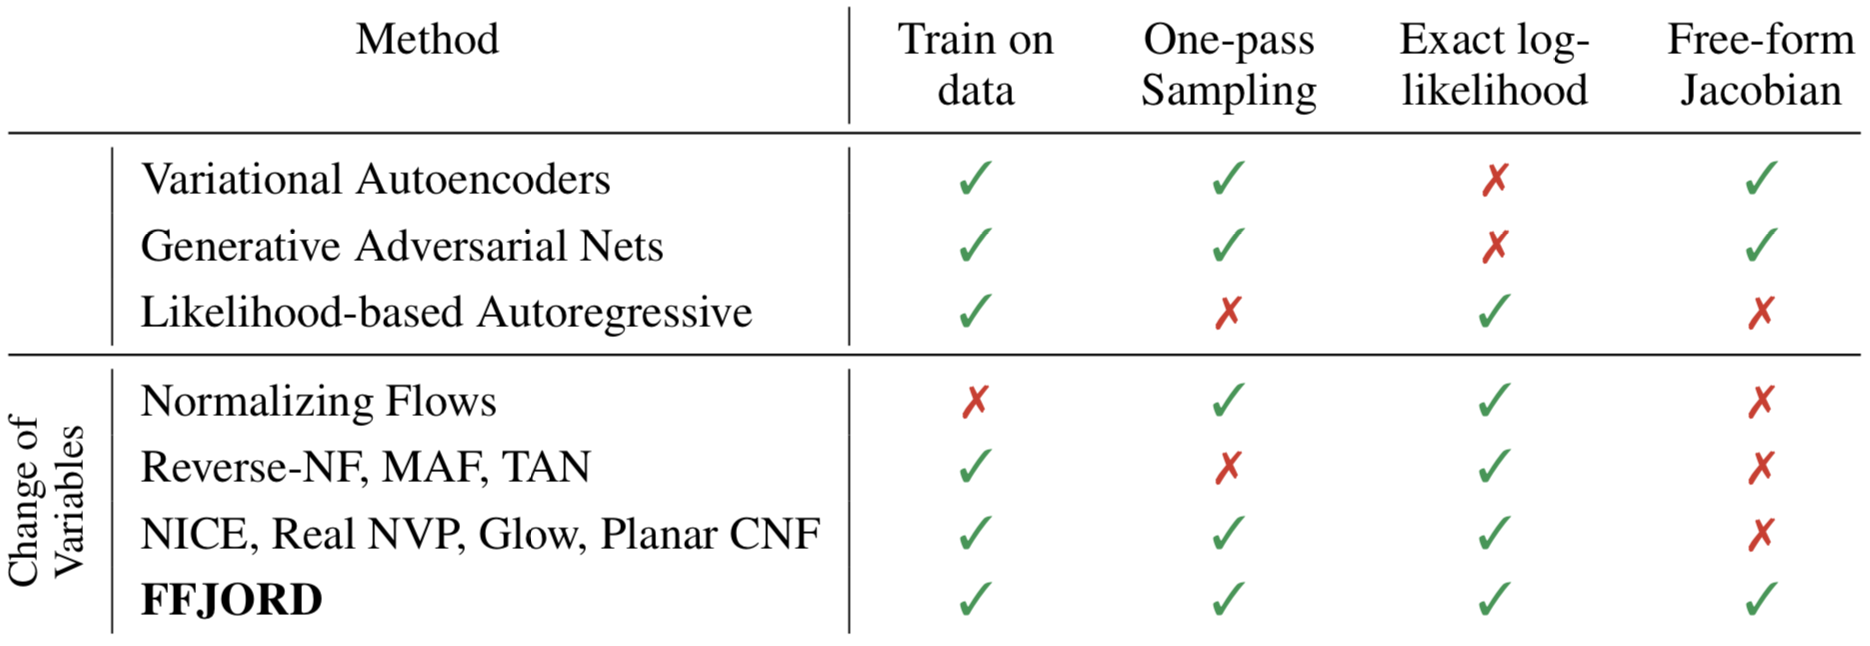
\includegraphics[width=\linewidth]{figs/flow_comparison.png}
		\end{figure}
	\end{block}
	\vspace{1cm}
	
	\hrule\medskip
	{\scriptsize \href{https://arxiv.org/abs/1810.01367}{https://arxiv.org/abs/1810.01367}} 
\end{frame}
%=======
\begin{frame}{FFJORD}
	\begin{block}{Density estimation}
		\begin{figure}
			\centering
			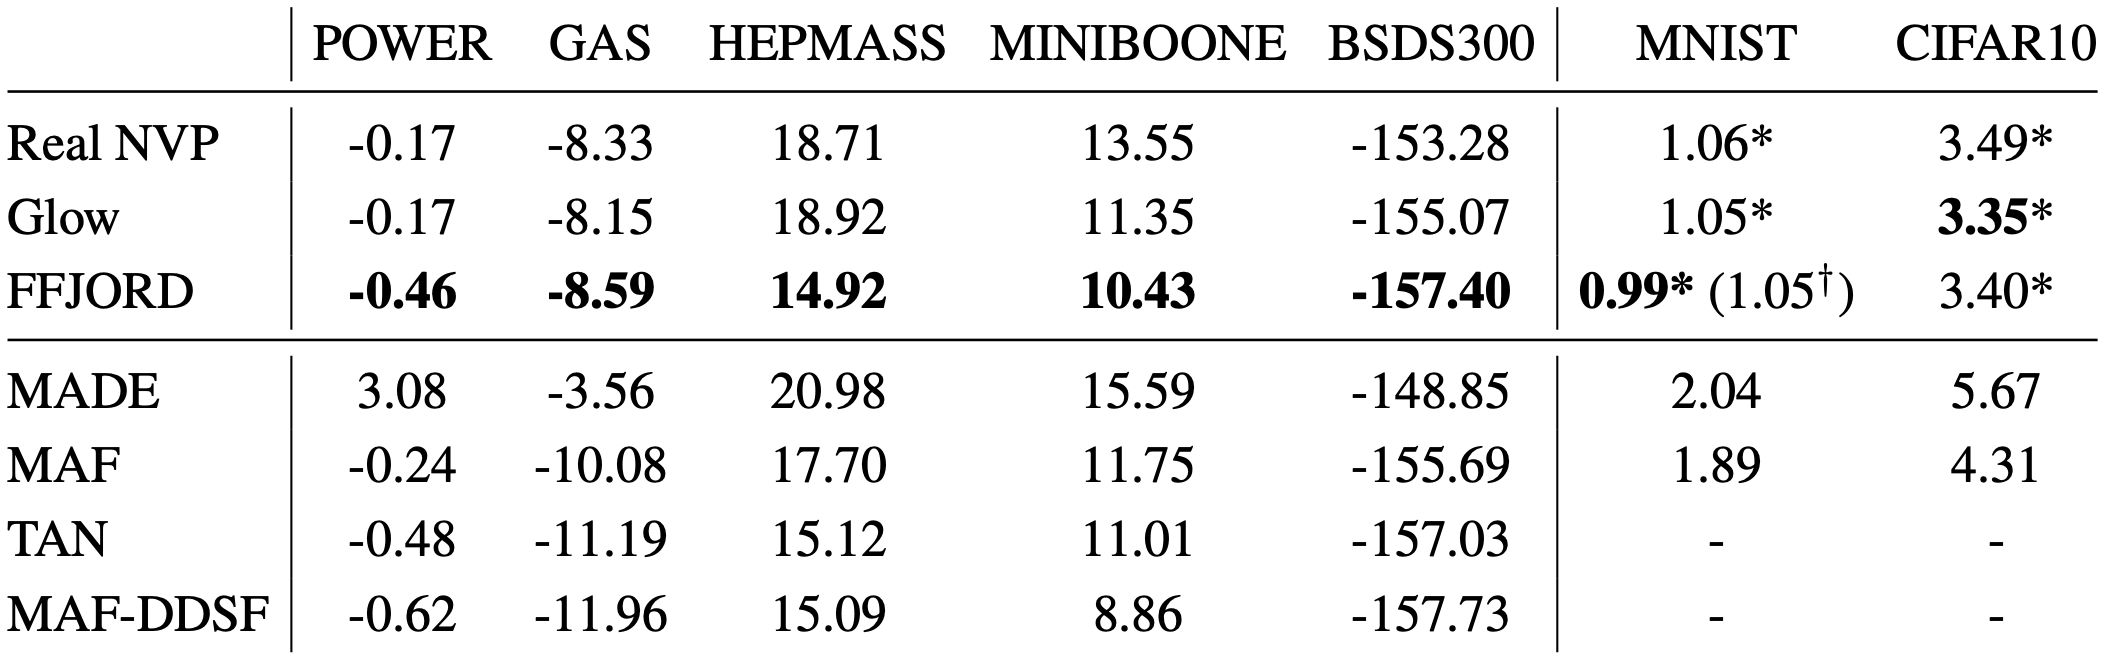
\includegraphics[width=0.8\linewidth]{figs/ffjord_results}
		\end{figure}
	\end{block}
	\begin{block}{Flows for variational inference}
		\begin{figure}
			\centering
			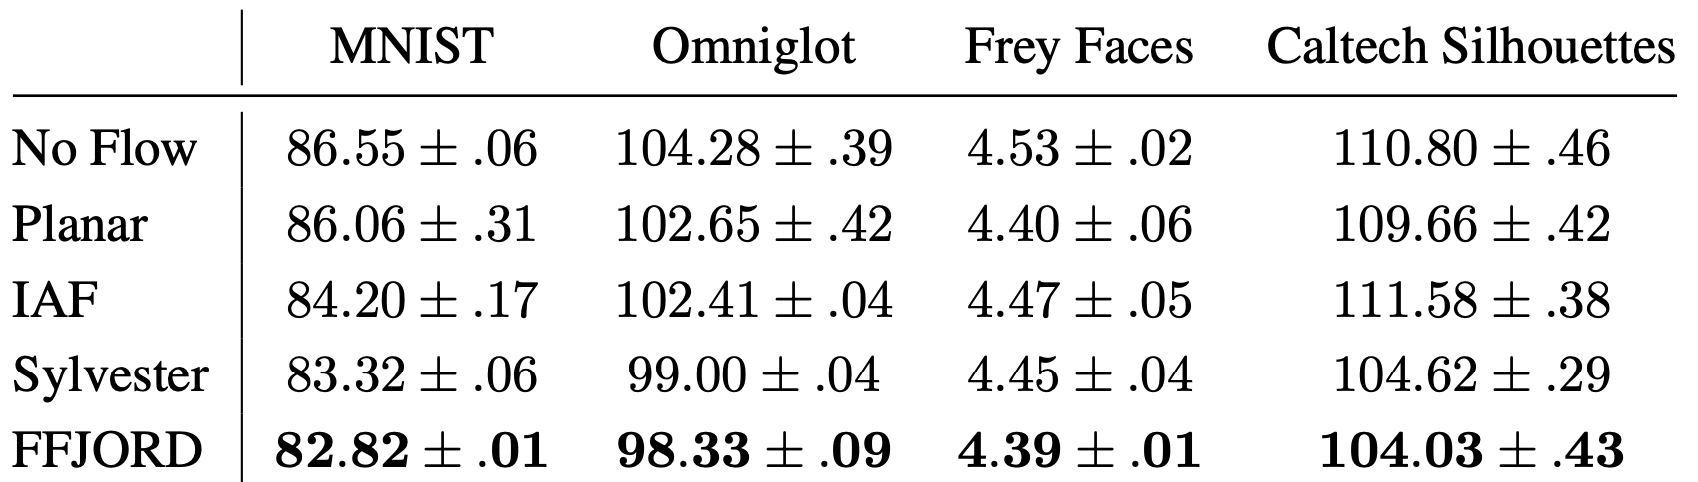
\includegraphics[width=0.8\linewidth]{figs/ffjord_vae}
		\end{figure}
	\end{block}
	\vfill
	\hrule\medskip
	{\scriptsize \href{https://arxiv.org/abs/1810.01367}{https://arxiv.org/abs/1810.01367}} 
\end{frame}
%=======
\begin{frame}{FFJORD}
\begin{figure}
    \centering
    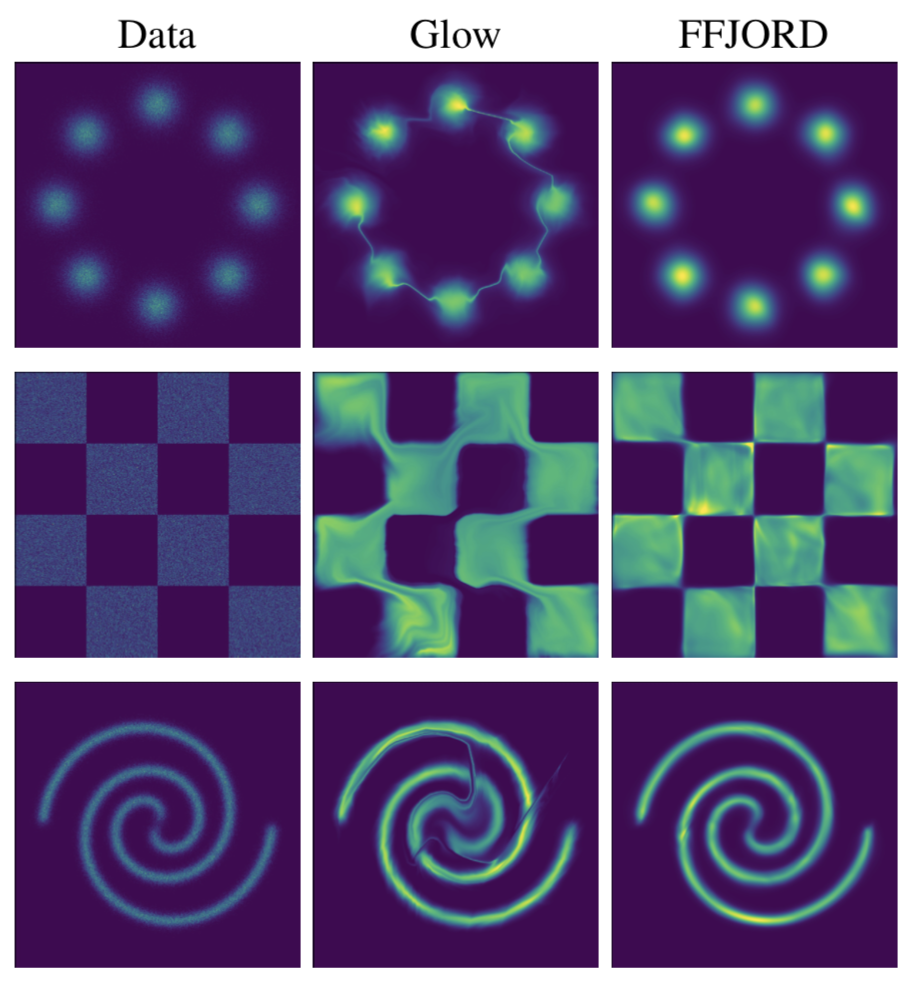
\includegraphics[width=0.6\linewidth]{figs/ffjord.png}
\end{figure}
\vfill
\hrule\medskip
{\scriptsize \href{https://arxiv.org/abs/1810.01367}{https://arxiv.org/abs/1810.01367}} 
\end{frame}
%=======
\begin{frame}{Discrete VAE}
	\begin{itemize}
		\item Before we have discussed VAE with \textbf{continuous} latent variables.
		\item VAE suffers from posterior collapse if the decoder too powerful (PixelVAE, VLAE tries to solve this problem).
		\item \textbf{Discrete} representations are potentially a more natural fit for many of the modalities.
		\item Powerful autoregressive models (like PixelCNNN) have been developed for modelling distributions over discrete variables.
		\item However, to construct the model with discrete representations is not so easy (e.g. variance of such estimators is a problem).
	\end{itemize}
	\vfill
	\hrule\medskip
	{\scriptsize \href{https://arxiv.org/abs/1711.00937}{https://arxiv.org/abs/1711.00937}} 
\end{frame}
%=======
\begin{frame}{Vector Quantized VAE}
	\begin{itemize}
		\item Latent embedding space $\{\be_j\}_{j=1}^K$, where $\be_j \in \bbR^D$, $K$ is the size of the discrete latent space.
		\item $\bz_e(\bx)$ is the encoder output.
		\item $z$ is the discrete random variable calculated by a nearest neighbour look-up using the shared embedding space. The posterior categorical distribution is defined as 
		\[
			q(z = k | \bx) = \begin{cases}
				1 , \quad \text{for } k = \argmin_j \| \bz_e(\bx) - \be_j \| \\
				0, \quad \text{otherwise}.
			\end{cases}
		\]
		
		\item VAE proposal distribution $q(z | \bx)$ is deterministic. If prior $p(z)$ is a uniform then $KL(q(z| \bx) || p(z))$ term in ELBO is constant (equals to $\log K$).
		\item Quantized representation is defined as follows
		\[
			\bz_q(\bx) = \be_k, \quad \text{where } k = \argmin_j \| \bz_e(\bx) - \be_j \| 
		\] 
		
	\end{itemize}
	\vfill
	\hrule\medskip
	{\scriptsize \href{https://arxiv.org/abs/1711.00937}{https://arxiv.org/abs/1711.00937}} 
\end{frame}
%=======
\begin{frame}{Vector Quantized VAE}
	\begin{figure}
		\centering
		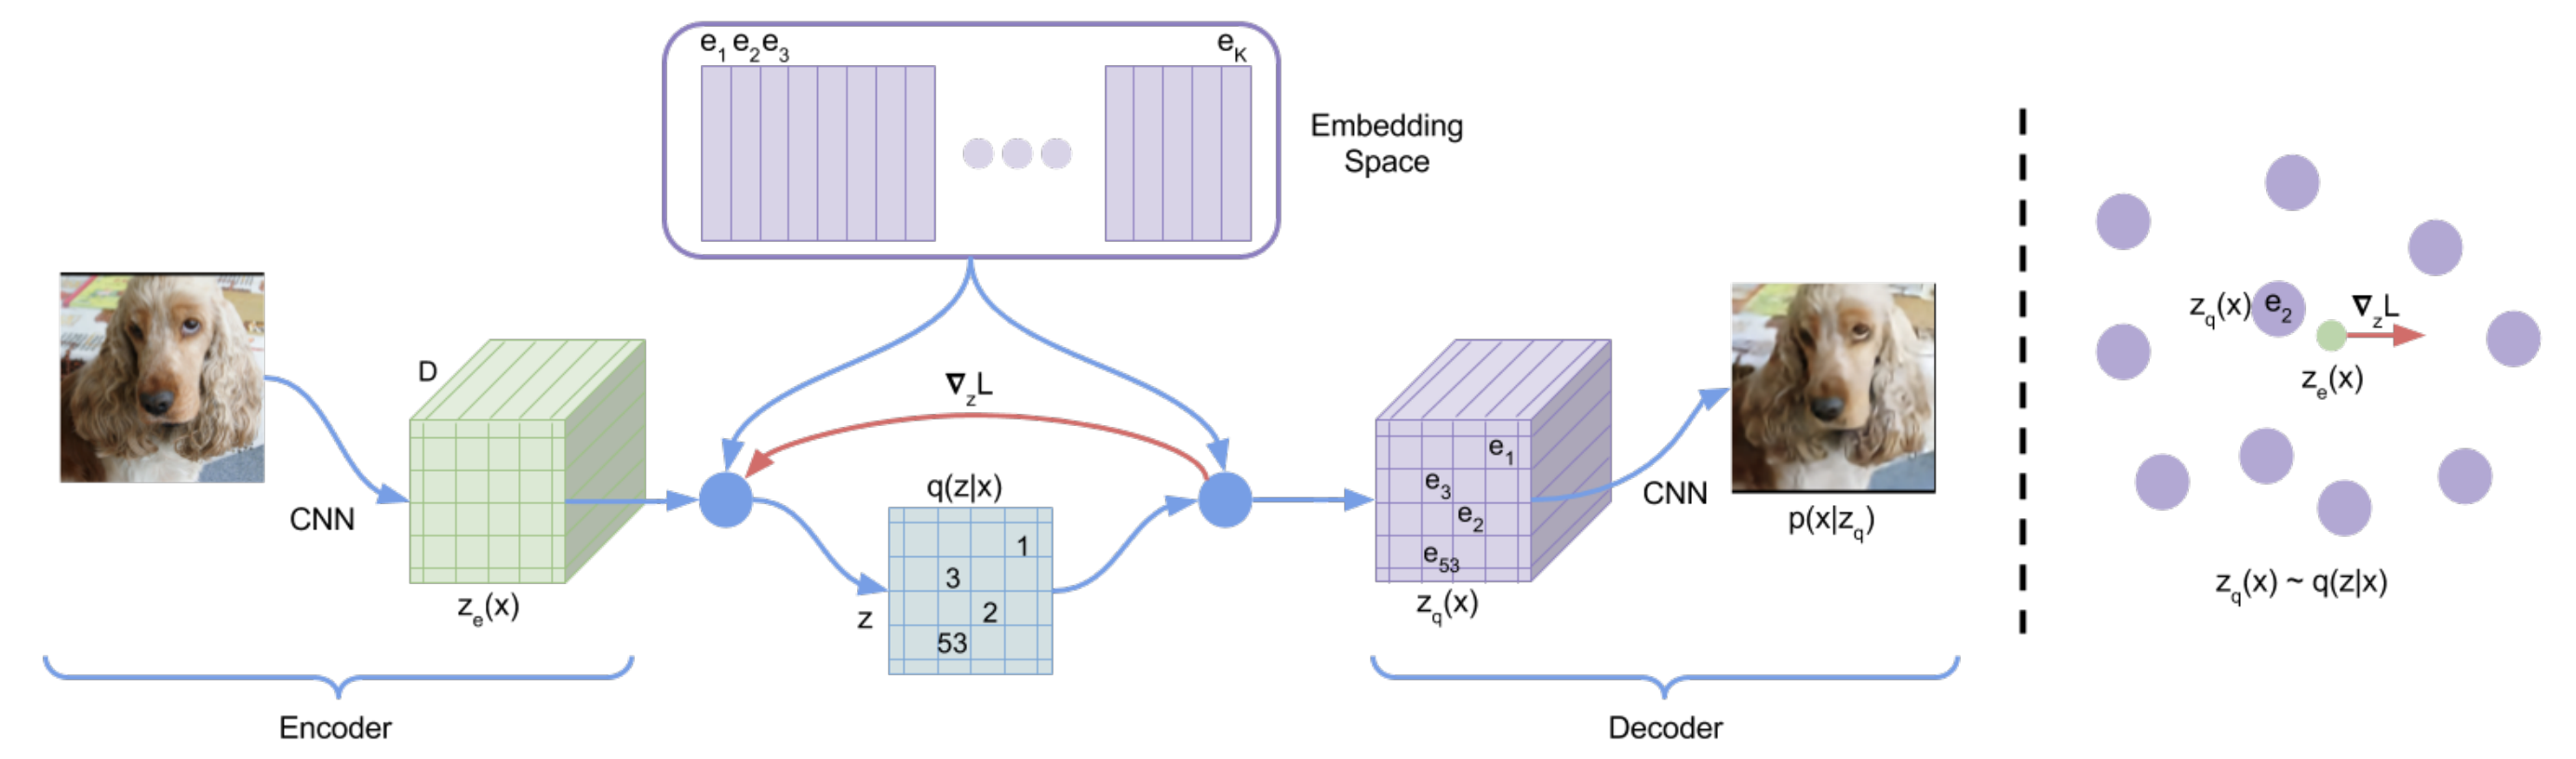
\includegraphics[width=\linewidth]{figs/vqvae}
	\end{figure}
	\begin{block}{Objective}
		\vspace{-0.3cm}
		\[
			\log p(\bx | \bz_q(\bx)) + \| \text{sg} (\bz_e(\bx)) - \bz_q(\bx) \| + \beta \| \bz_e(\bx) - \text{sg}(\bz_q(\bx)) \|
		\]
	\end{block}
	\begin{itemize}
		\item Quantization operation is not differentiable.
		\item Straight-through gradient estimation is used to backpropagate the quantization operation.
	\end{itemize}
	\vfill
	\hrule\medskip
	{\scriptsize \href{https://arxiv.org/abs/1711.00937}{https://arxiv.org/abs/1711.00937}} 
\end{frame}
%=======
\begin{frame}{Vector Quantized VAE}
	\begin{itemize}
		\item The prior distribution over the discrete latents $p(\bz)$ is a categorical distribution.
		\item It could be made autoregressive by depending on other $\bz$ in the feature map. 
		\item Whilst training the VQ-VAE, the prior is kept constant and uniform. 
		\item After training, fit an autoregressive distribution (using PixelCNN) over $\bz$.
	\end{itemize}
	\begin{figure}
		\centering
		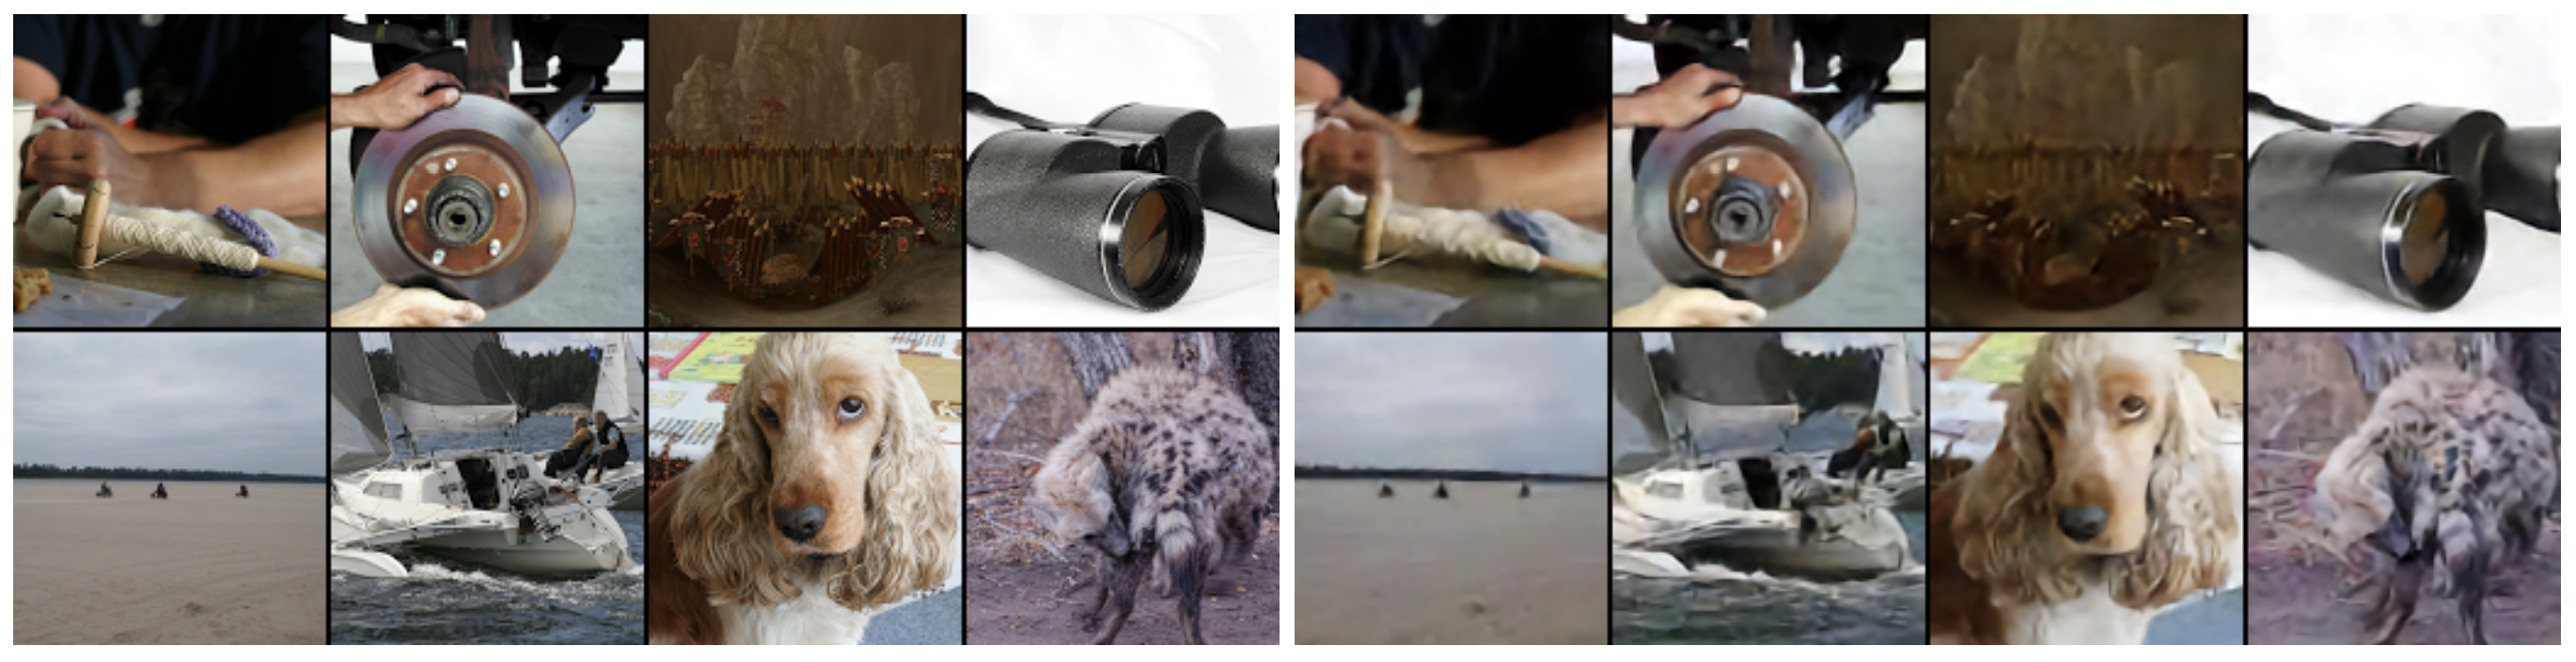
\includegraphics[width=\linewidth]{figs/vqvae_results}
	\end{figure}
	\vfill
	\hrule\medskip
	{\scriptsize \href{https://arxiv.org/abs/1711.00937}{https://arxiv.org/abs/1711.00937}} 
\end{frame}
%=======
\begin{frame}{Vector Quantized VAE-2}
	\begin{itemize}
		\item Use multi-scale hierarchical model.
		\item Use autoregressive prior model in each scale of the hierarchy.
		\item Improve autoregressive prior (PixelSNAIL with self-attention in bottom layer, PixelCNN++ in bottom layer).
		\item Train the encoder and decoder at the first stage, train the priors at the second stage.
	\end{itemize}
	\begin{figure}
		\centering
		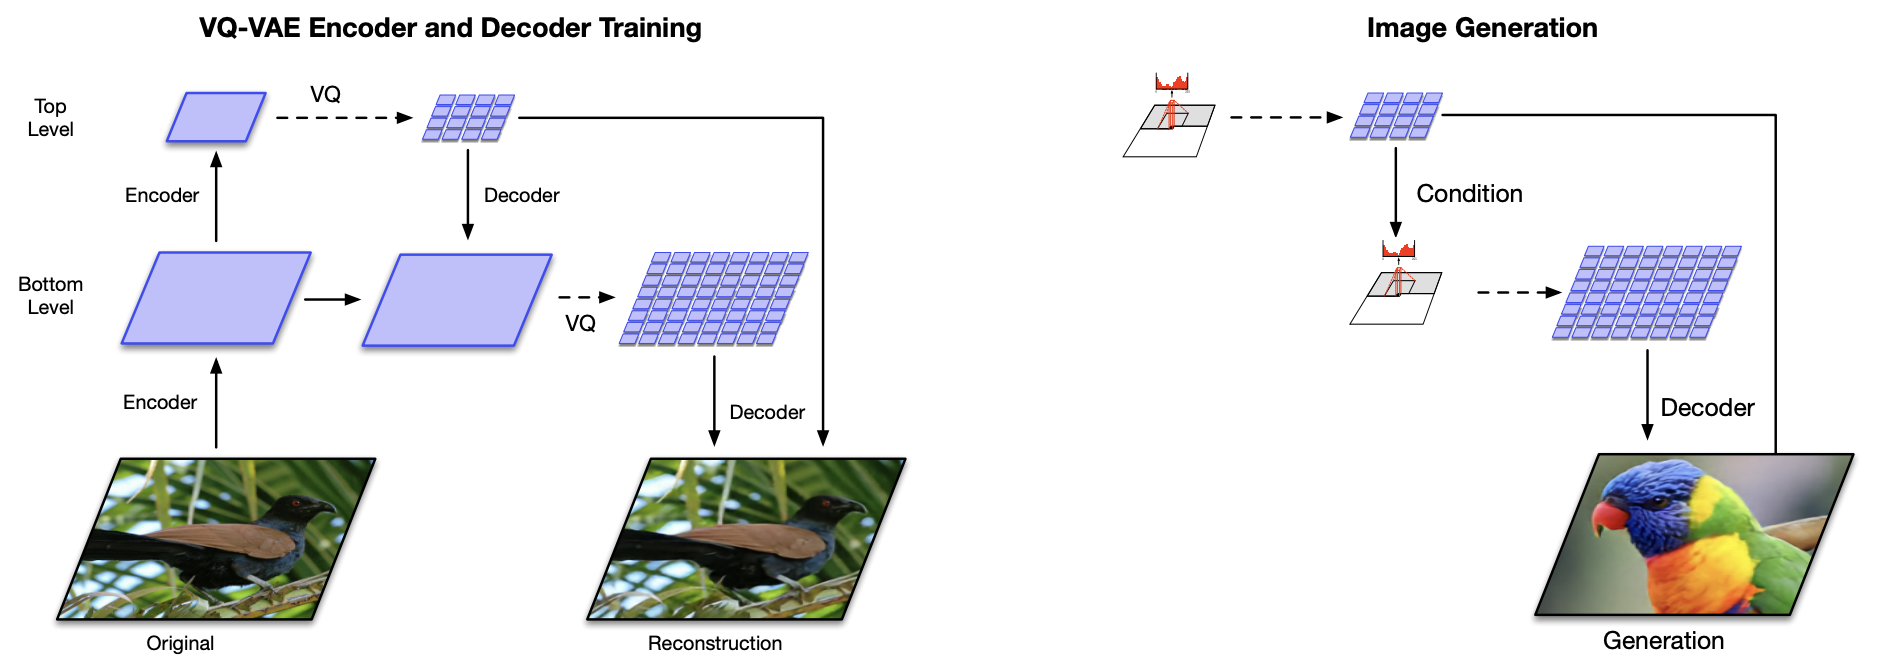
\includegraphics[width=\linewidth]{figs/vqvae2}
	\end{figure}
	\vfill
	\hrule\medskip
	{\scriptsize \href{https://arxiv.org/abs/1906.00446}{https://arxiv.org/abs/1906.00446}} 
\end{frame}
%=======
\begin{frame}{Vector Quantized VAE-2}
		\begin{figure}
			\centering
			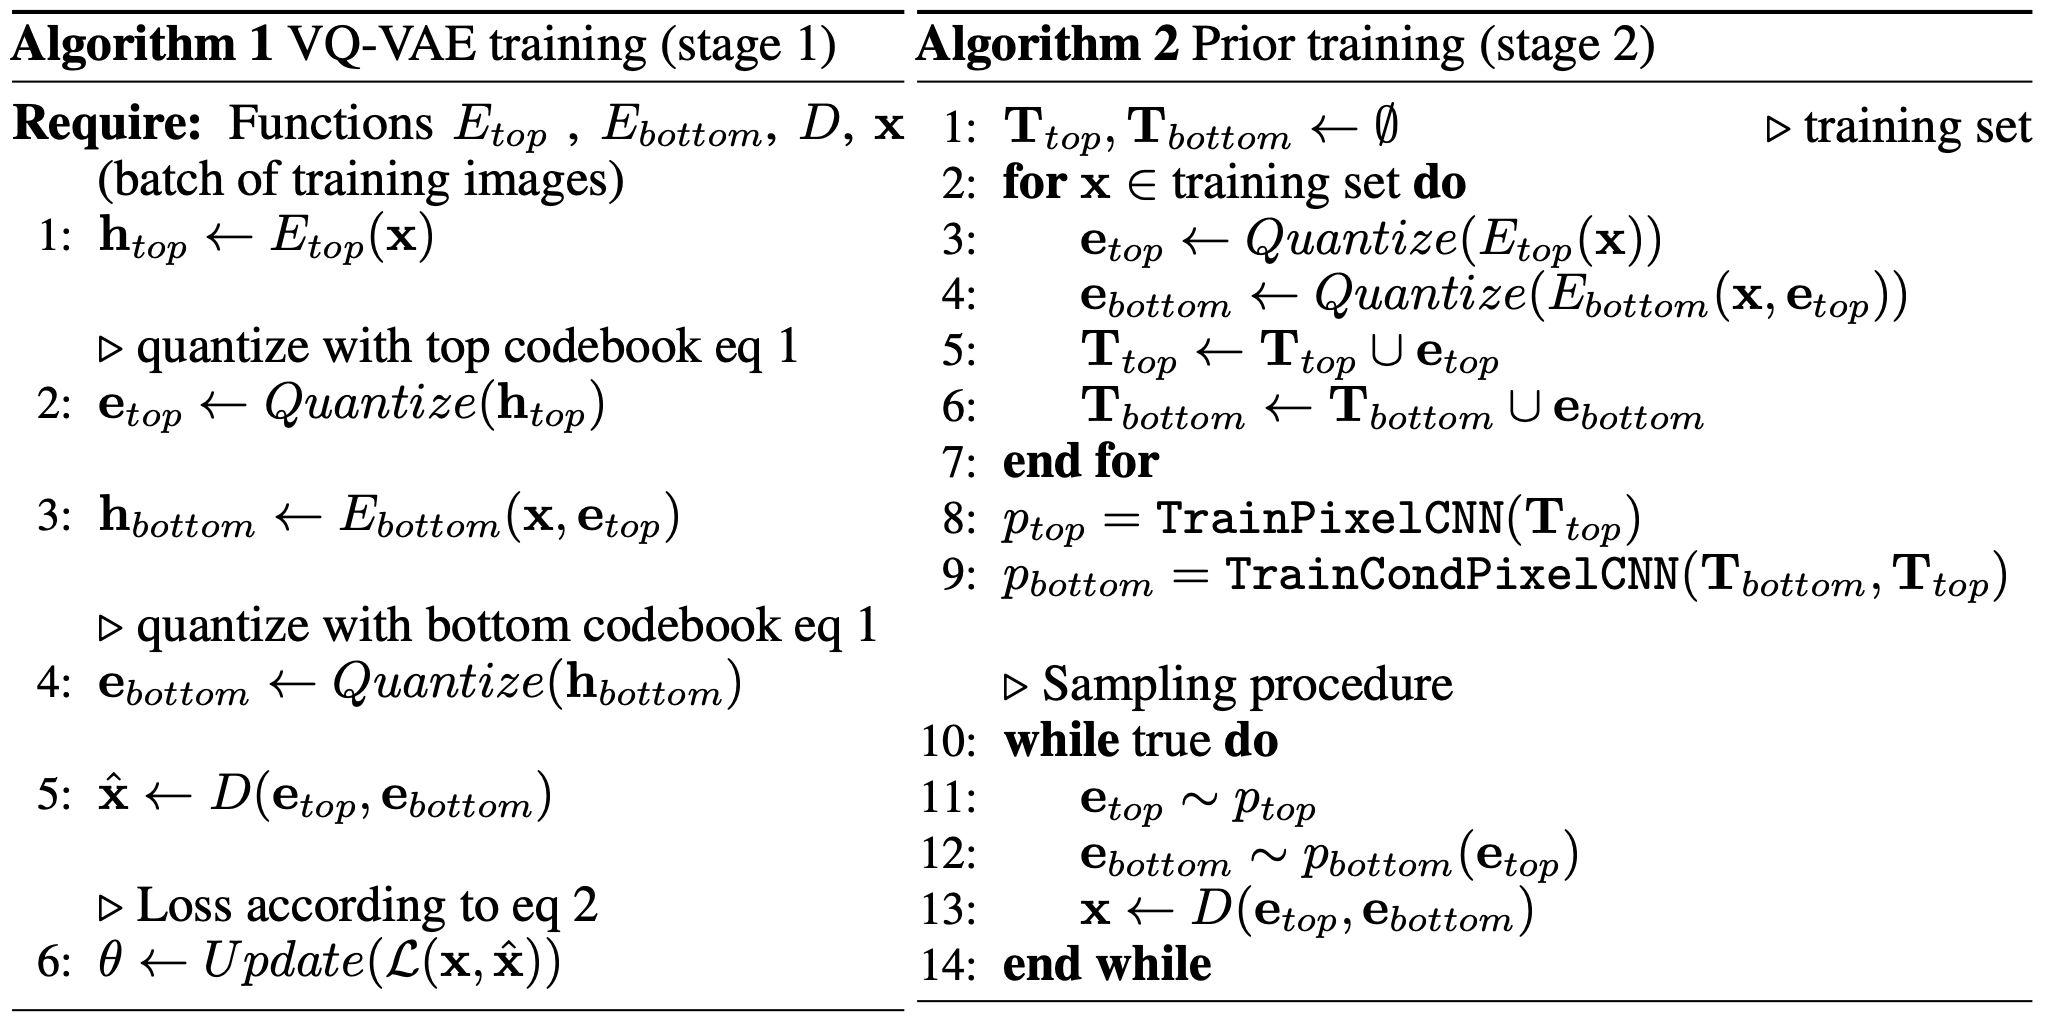
\includegraphics[width=0.9\linewidth]{figs/vqvae2_pseudo}
		\end{figure}
		\begin{figure}
			\centering
			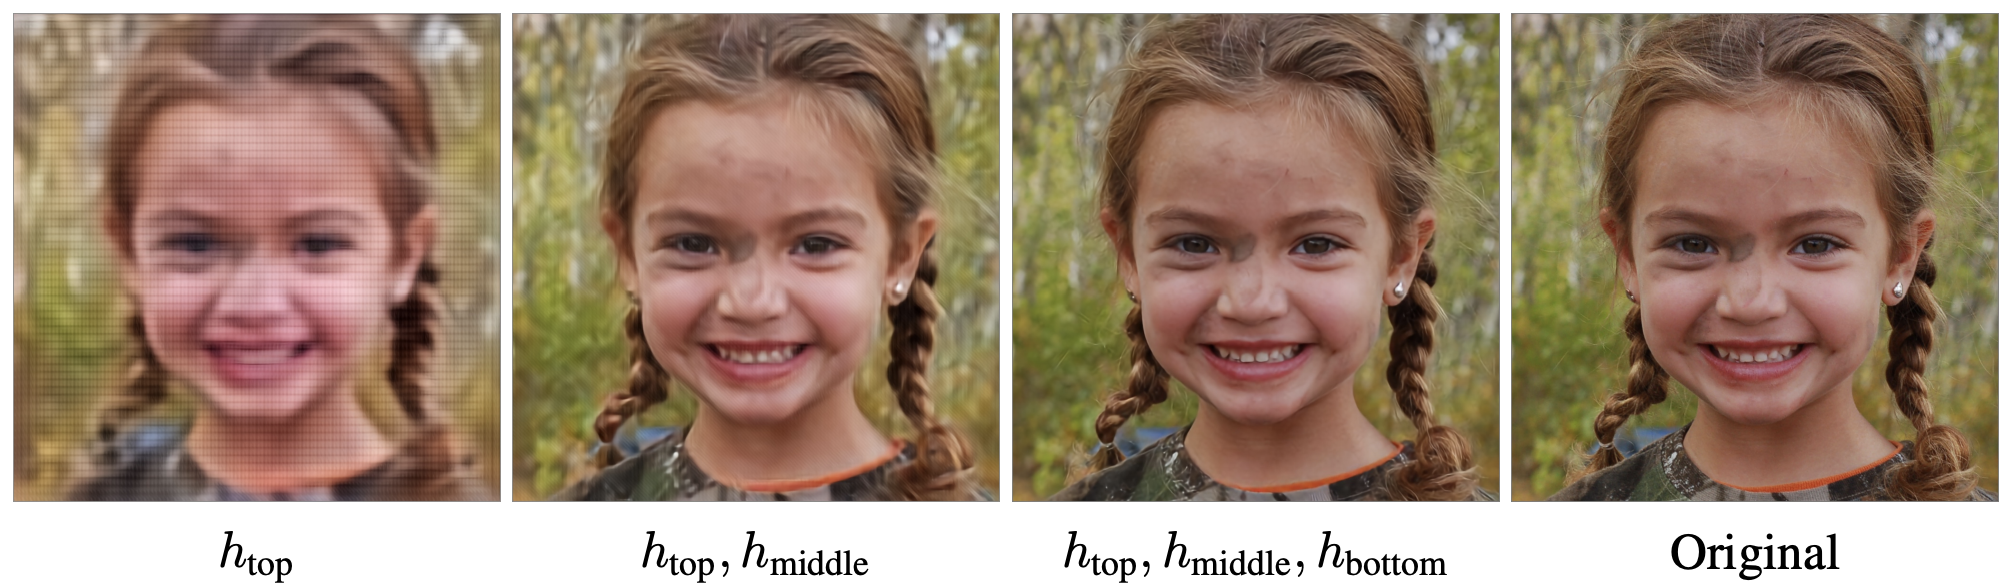
\includegraphics[width=0.85\linewidth]{figs/vqvae2_latents}
		\end{figure}
	\vfill
	\hrule\medskip
	{\scriptsize \href{https://arxiv.org/abs/1906.00446}{https://arxiv.org/abs/1906.00446}} 
\end{frame}
%=======
\begin{frame}{Vector Quantized VAE-2}
	\begin{block}{FFHQ 1024x1024}
	\begin{figure}
		\centering
		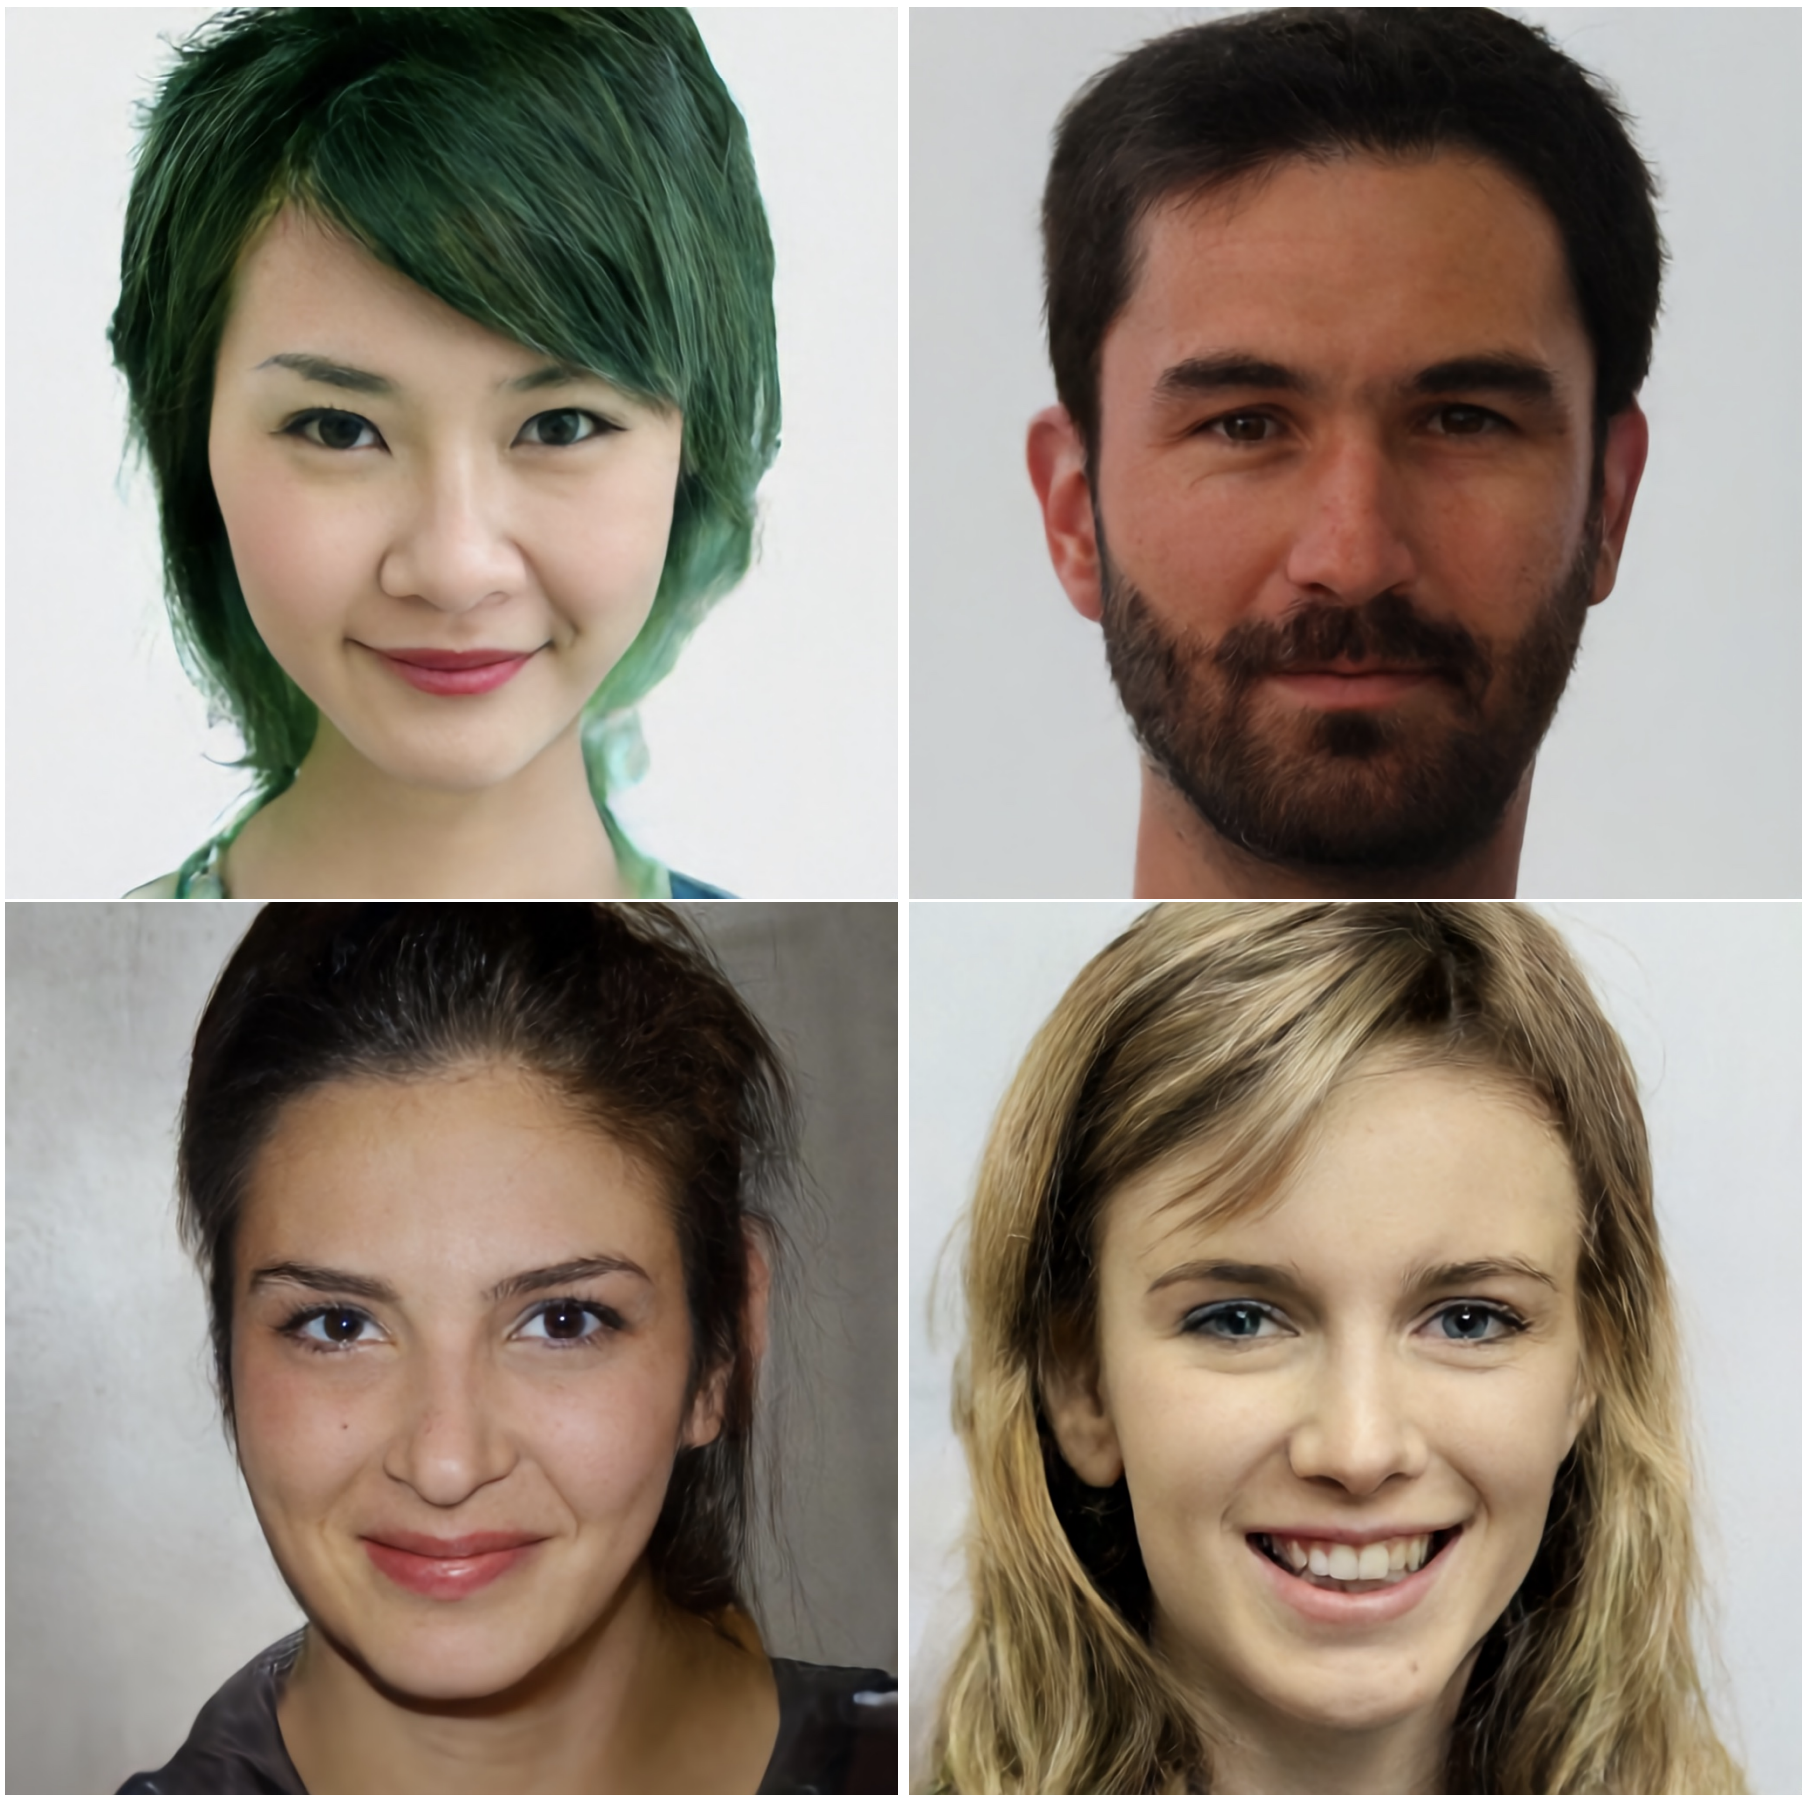
\includegraphics[width=0.63\linewidth]{figs/vqvae2_faces}
	\end{figure}
	\end{block}
	\vfill
	\hrule\medskip
	{\scriptsize \href{https://arxiv.org/abs/1906.00446}{https://arxiv.org/abs/1906.00446}} 
\end{frame}
%=======
\begin{frame}{Vector Quantized VAE-2}
	\begin{figure}
		\centering
		\includegraphics[width=0.7\linewidth]{figs/vqvae2_diversity}
	\end{figure}
	\vfill
	\hrule\medskip
	{\scriptsize \href{https://arxiv.org/abs/1906.00446}{https://arxiv.org/abs/1906.00446}} 
\end{frame}
%=======
\begin{frame}{Feature Quantized GAN}
	\begin{itemize}
		\item GAN tries to find Nash equilibrium, minibatch training is unstable. GAN relies heavily on the minibatch statistics.
		\item Lots of feature matching strategies were proposed to stabilize the training. 
	\end{itemize}
	\begin{block}{Feature quantized GAN discriminator}
		\[
			D(\bx) = f_{\bw_T} \circ f_{\bw_B}(\bx) \quad \Rightarrow \quad D(\bx) = f_{\bw_T} \circ f_Q \circ f_{\bw_B}(\bx). 
		\]
	\end{block}
	Here $f_Q$ is a vector quantization operation.
	\begin{figure}
		\centering
		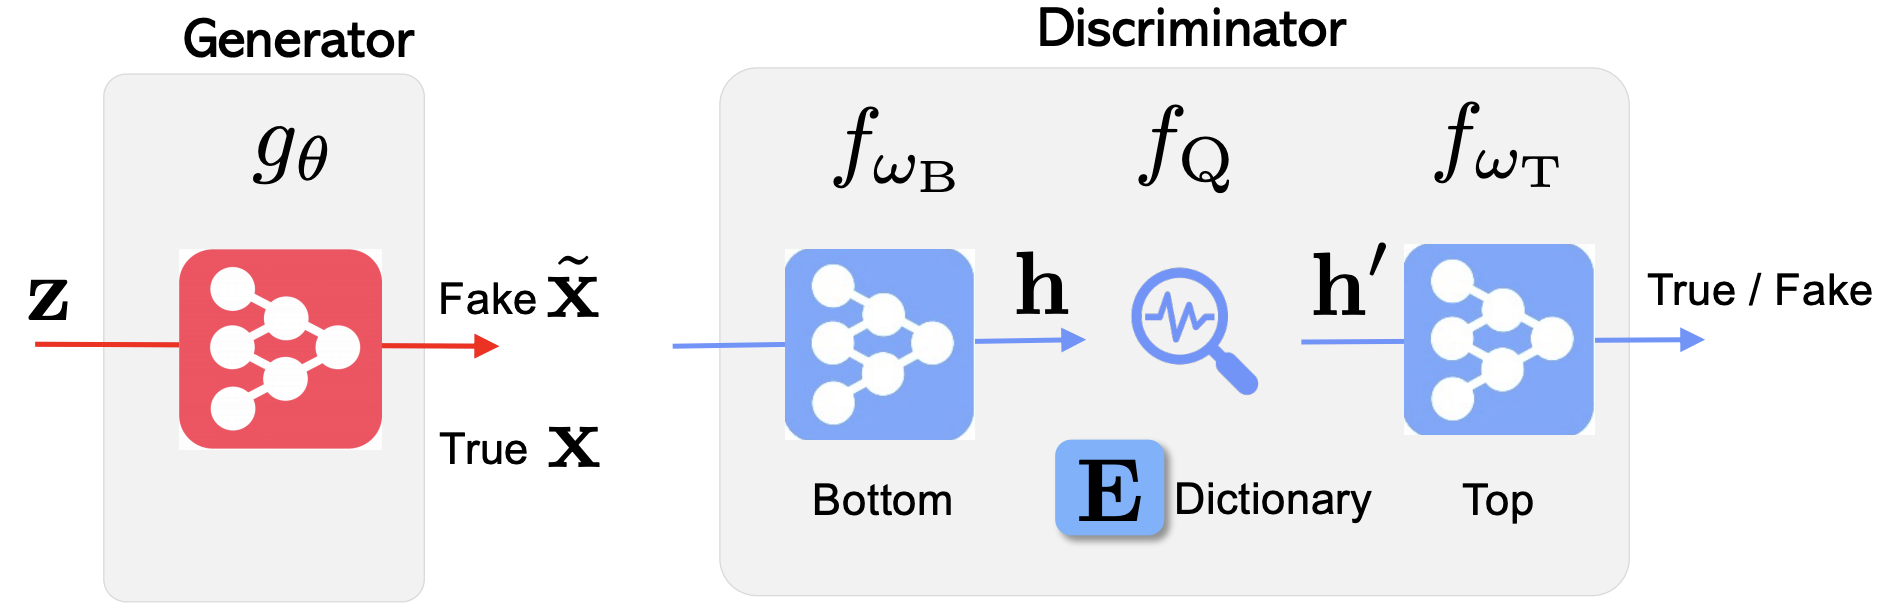
\includegraphics[width=0.7\linewidth]{figs/fqgan}
	\end{figure}
	\vfill
	\hrule\medskip
	{\scriptsize \href{https://arxiv.org/abs/2004.02088}{https://arxiv.org/abs/2004.02088}} 
\end{frame}
%=======
\begin{frame}{Feature Quantized GAN}
	\begin{block}{Quantization procedure}
		\begin{minipage}[t]{0.65\columnwidth}
			\begin{figure}
				\centering
				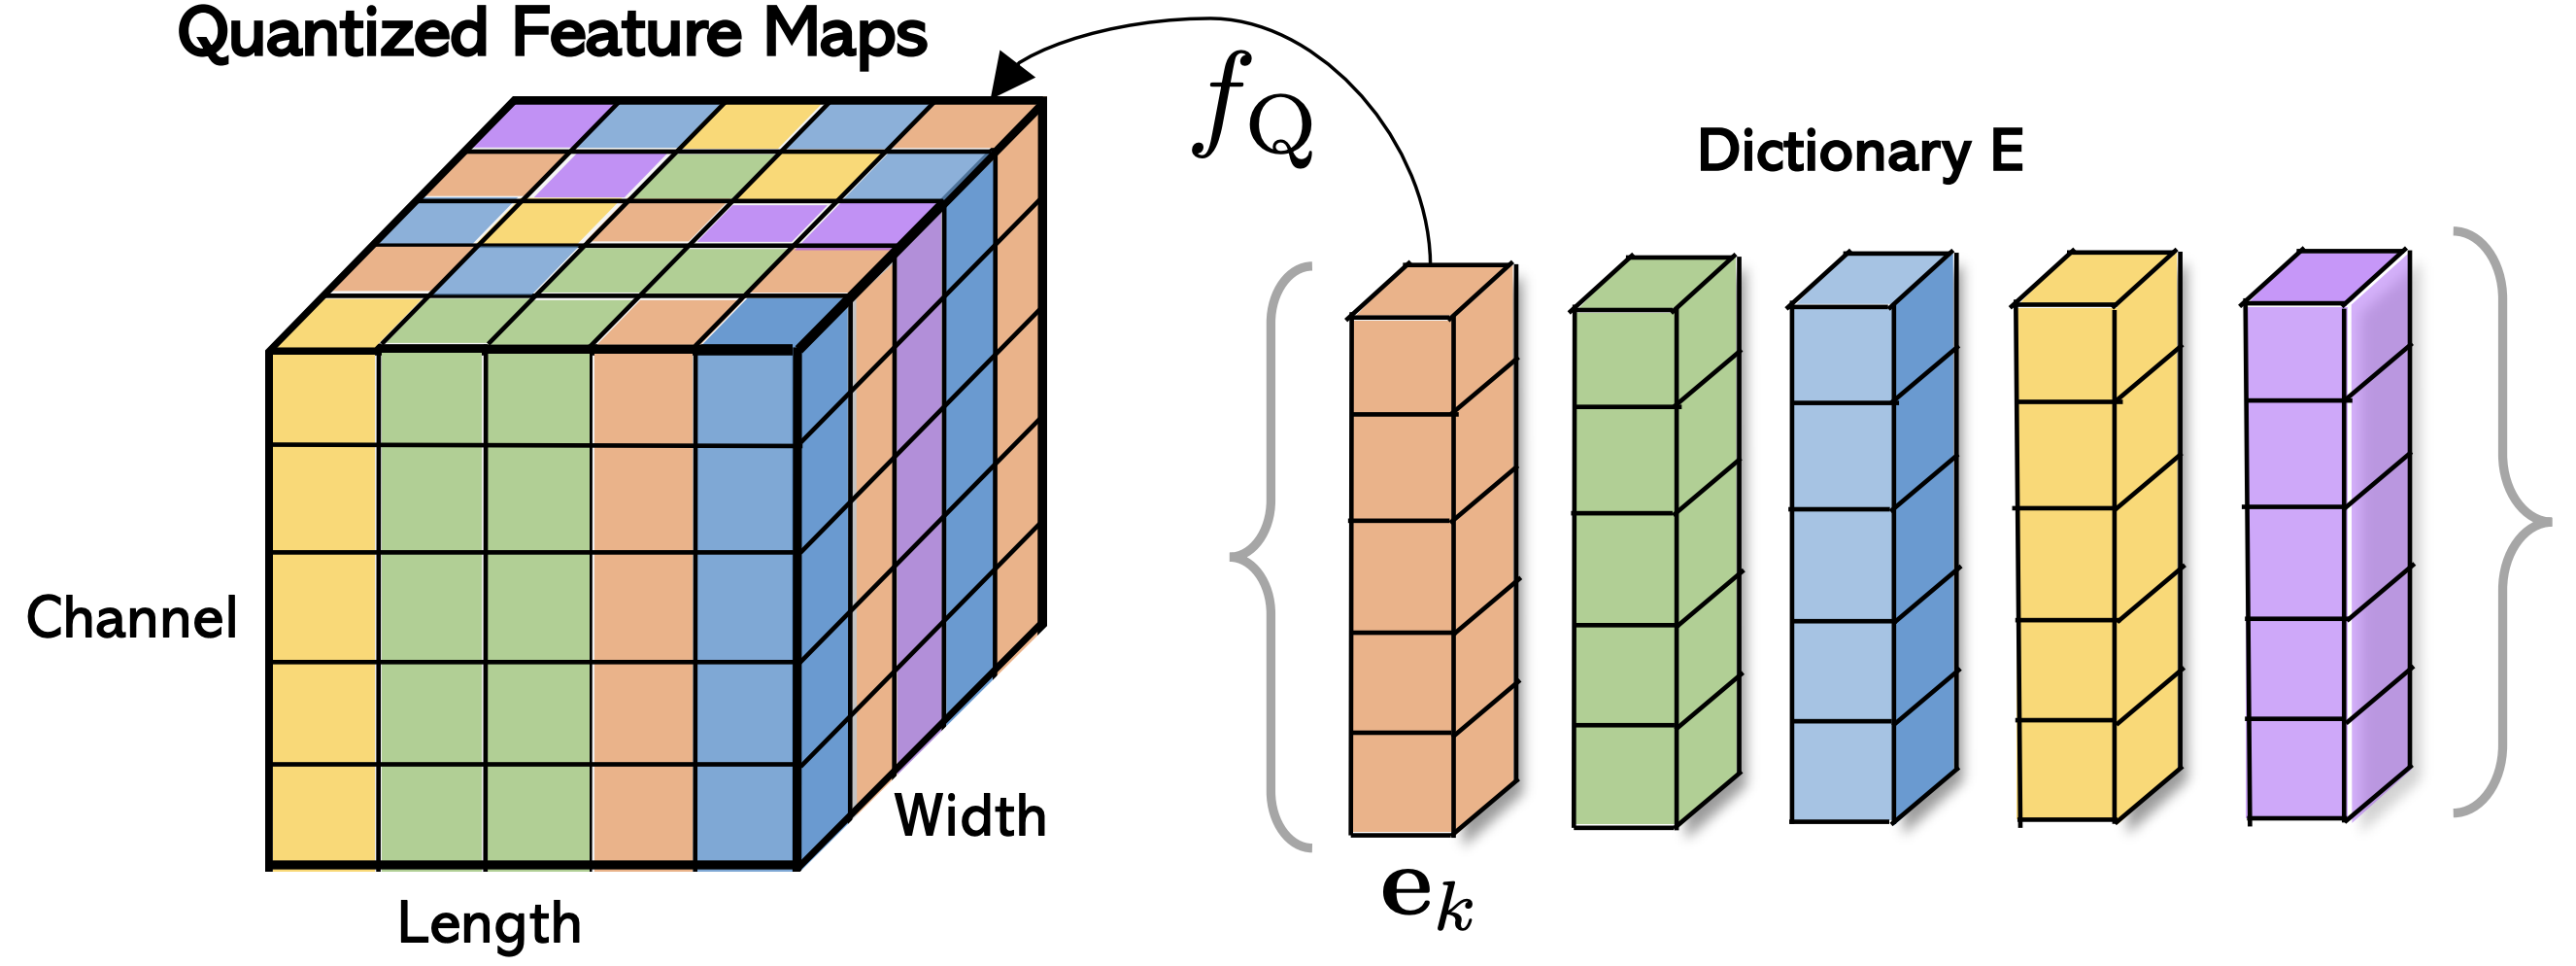
\includegraphics[width=\linewidth]{figs/fqgan_cnn.png}
			\end{figure}
		\end{minipage}%
		\begin{minipage}[t]{0.35\columnwidth}
			\begin{figure}
				\centering
				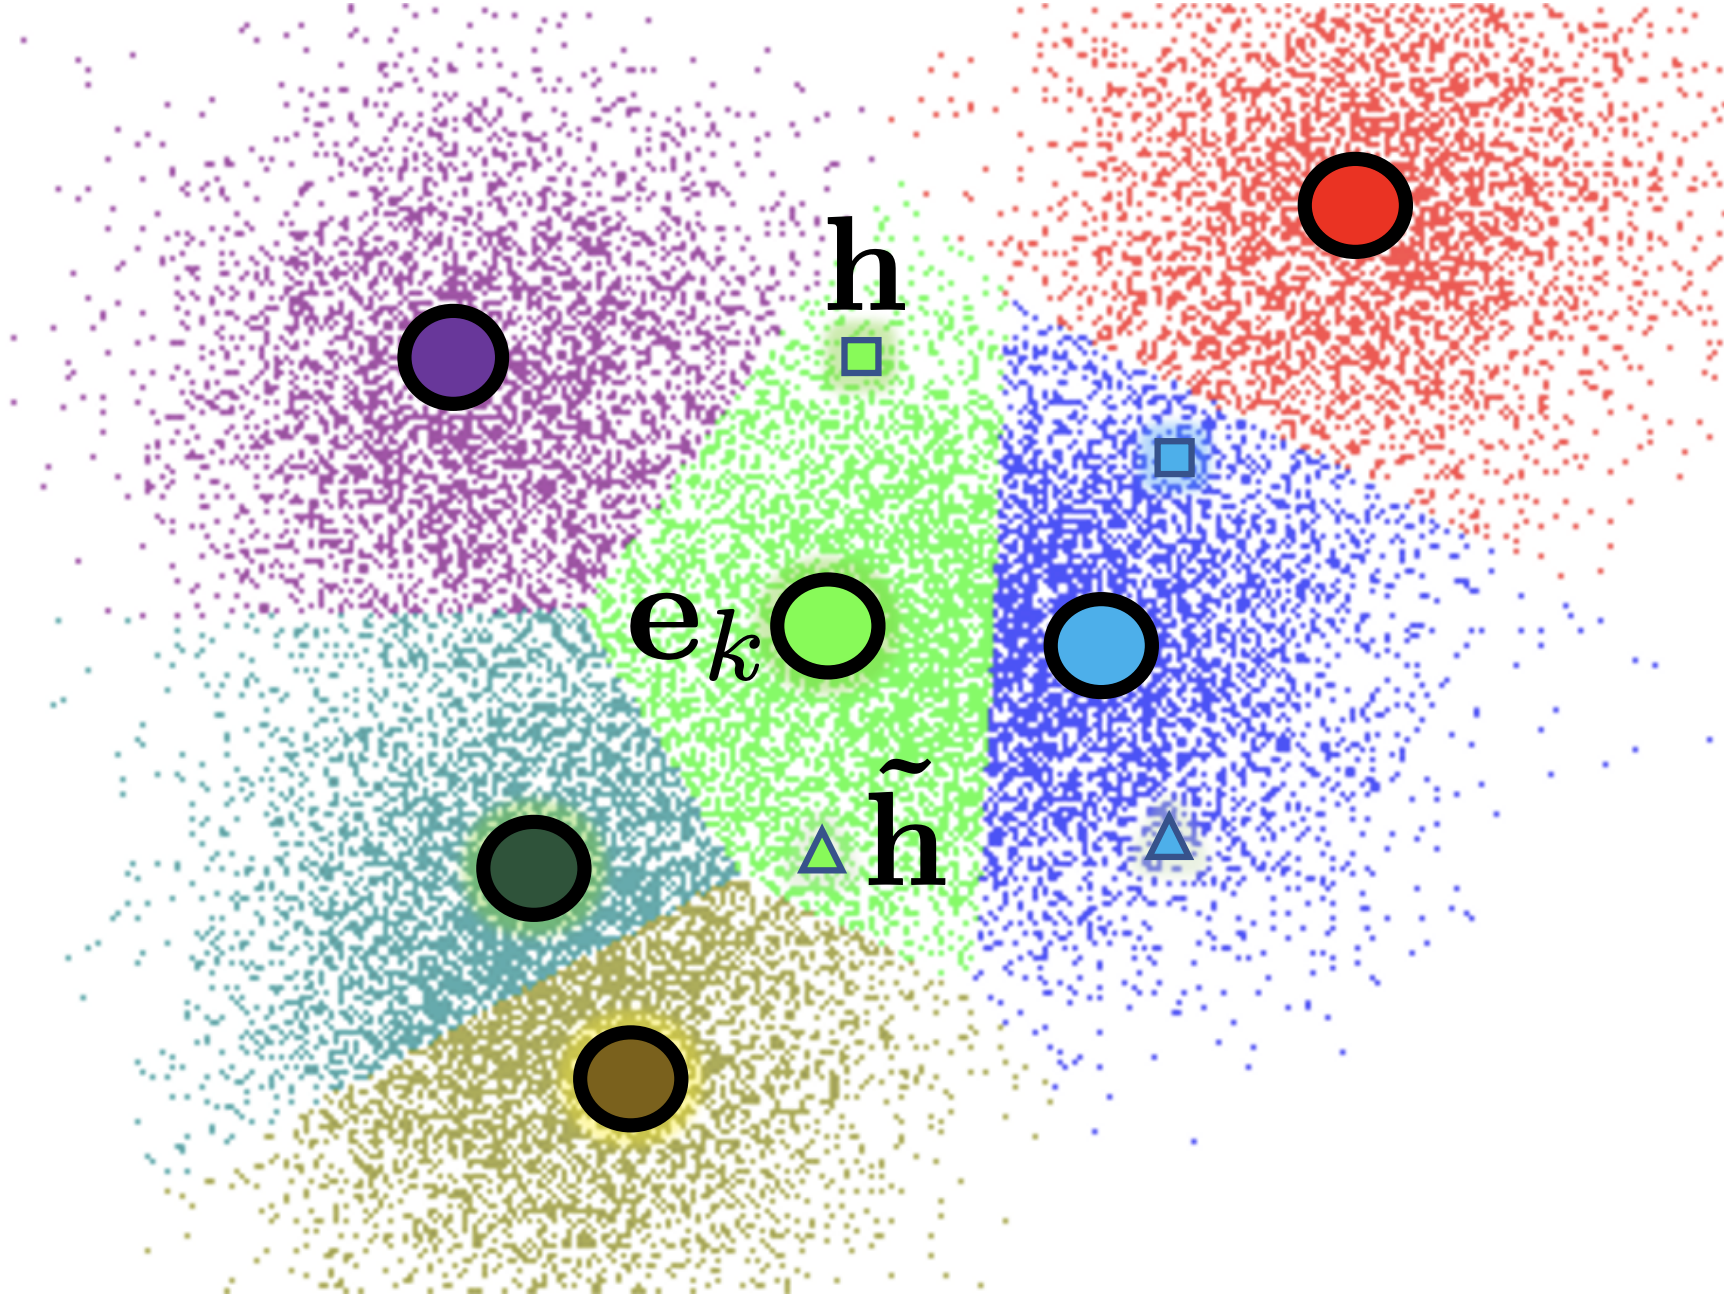
\includegraphics[width=0.9\linewidth]{figs/fqgan_lookup}
			\end{figure}
		\end{minipage}
	\end{block}
	\begin{block}{Quantized features}
		\begin{figure}
			\centering
			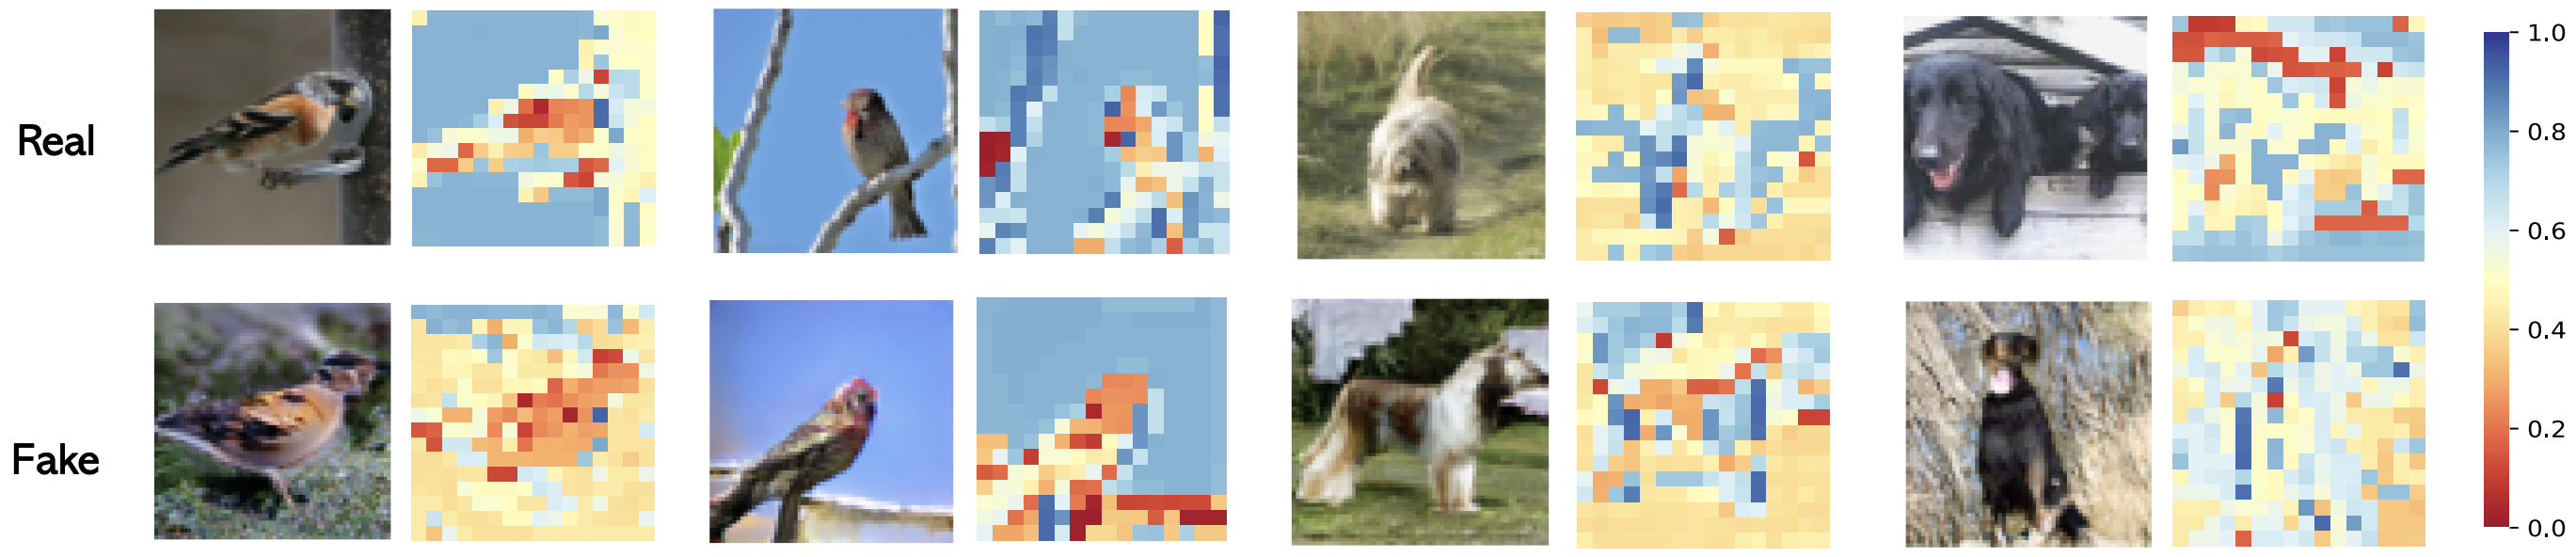
\includegraphics[width=\linewidth]{figs/fqgan_features}
		\end{figure}
	\end{block}
	\vfill
	\hrule\medskip
	{\scriptsize \href{https://arxiv.org/abs/2004.02088}{https://arxiv.org/abs/2004.02088}} 
\end{frame}
%=======
\begin{frame}{Feature Quantized GAN}
		\begin{minipage}[t]{0.45\columnwidth}
			\begin{block}{ImageNet-1000}
				\begin{figure}
					\centering
					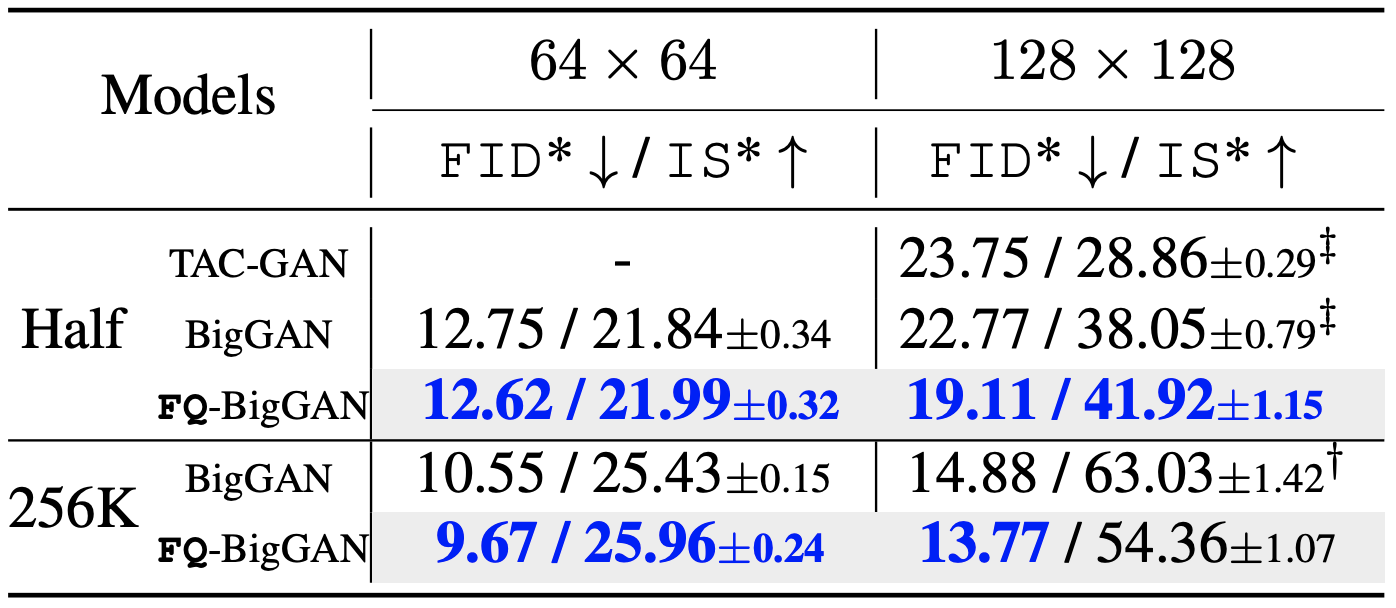
\includegraphics[width=\linewidth]{figs/fqgan_results1.png}
				\end{figure}
			\end{block}
			\begin{block}{FFHQ}
				\begin{figure}
					\centering
					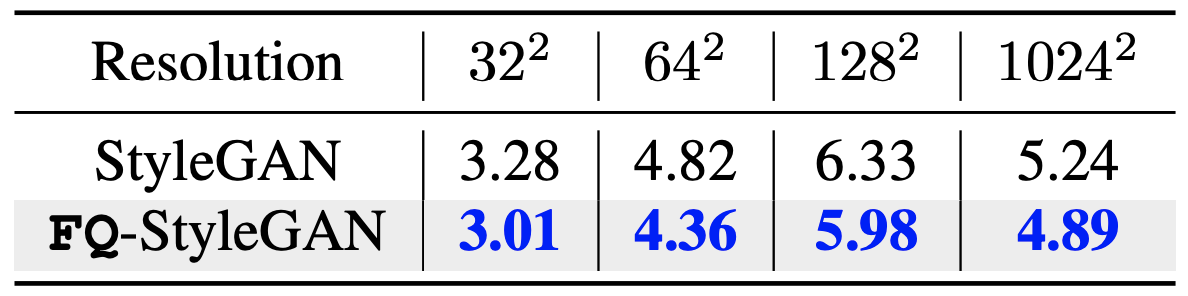
\includegraphics[width=\linewidth]{figs/fqgan_results2.png}
				\end{figure}
			\end{block}
		\end{minipage}%
		\begin{minipage}[t]{0.55\columnwidth}
			\begin{block}{Per class metrics for ImageNet}
				\begin{figure}
					\centering
					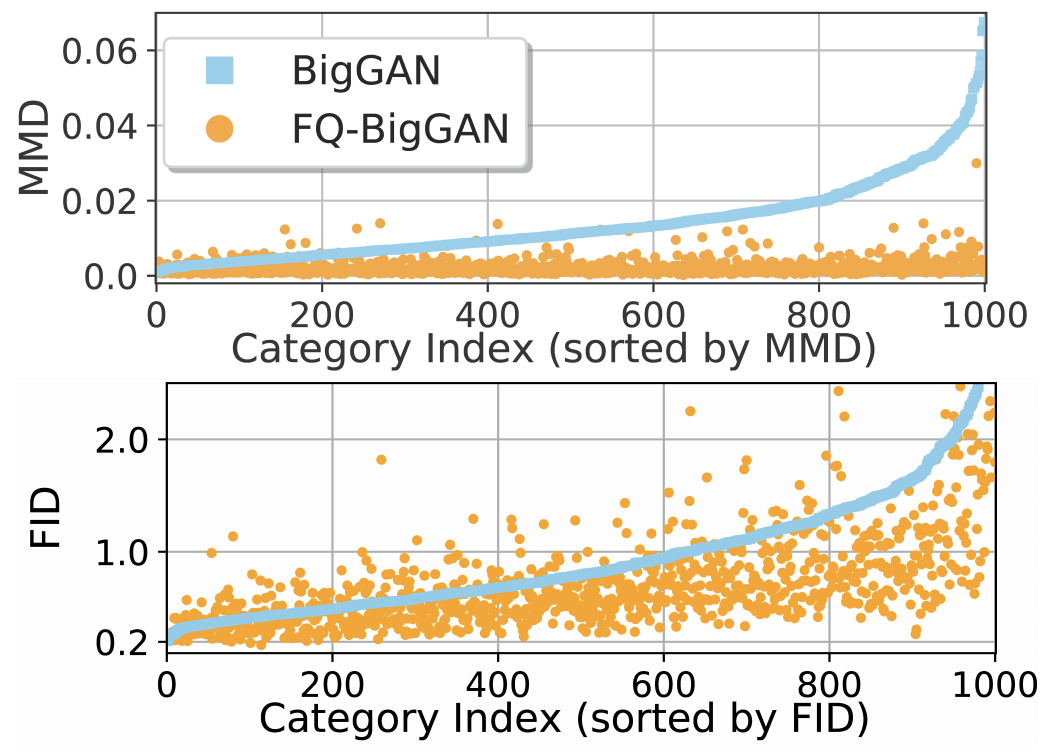
\includegraphics[width=\linewidth]{figs/fqgan_results3}
				\end{figure}
			\end{block}
		\end{minipage}
	\vspace{0.8cm}
	
	\hrule\medskip
	{\scriptsize \href{https://arxiv.org/abs/2004.02088}{https://arxiv.org/abs/2004.02088}} 
\end{frame}
%=======
\begin{frame}{References}
{\tiny
\begin{itemize}
    \item Neural Ordinary Differential Equations \\
    \href{https://arxiv.org/abs/1806.07366}{https://arxiv.org/abs/1806.07366} \\
    \textbf{Summary:} New interpretation of resnets as special case of ode. 
    Discrete sequence of layers  are replaced with continuous dynamic. ODESolver is used for backpropagation. Pontryagin theorem gives the analog of the chain rule. Continuous version \\ of normalizing flow is constructed.
    
    \item \textbf{FFJORD:} Free-form Continuous Dynamics for Scalable Reversible Generative Models \\
    \href{https://arxiv.org/abs/1810.01367}{https://arxiv.org/abs/1810.01367} \\
    \textbf{Summary:} Continuous version of NF is investigated. 
    Jacobian computation cost is reduced to O(D) by using Hutchinson’s \\ trace estimator. 
    
    \item \textbf{VQ-VAE:} Neural discrete representation learning \\
    \href{https://arxiv.org/abs/1711.00937}{https://arxiv.org/abs/1711.00937} \\
    \textbf{Summary:} Discrete latent representation for VAE. Nearest neighbor lookup table quantization is used. Learned powerful PixelCNN prior in the latent space.
    
    \item \textbf{VQ-VAE-2:} Generating Diverse High-Fidelity Images with VQ-VAE-2 \\
    \href{https://arxiv.org/abs/1906.00446}{https://arxiv.org/abs/1906.00446} \\
    \textbf{Summary:} The extension of VQ-VAE model for generating highly realistic images (comparable with sota gans). Use \\ hierarchical latent representation with PixelSnail prior. Comparison with BigGan.
    
    \item \textbf{FQ-VAE:} Feature Quantization Improves GAN Training \\
    \href{https://arxiv.org/abs/2004.02088}{https://arxiv.org/abs/2004.02088} \\
    \textbf{Summary:} Lots of "feature matching" techniques for GANN was introduced to stabilize training. Vector quantization has a proporty of implicit feature matching. Adding vector quantization module to GAN discriminator improves quality.
\end{itemize}
}
\end{frame}
\end{document} 